%!TEX root = draft.tex
%\newcommand{\seqPQ}{\mathsf{SeqPQ}}

\section{Compositionality of \CRDTLin{}}
\label{sec:compositionality}

%\textblue{
%This section should give three results of the form: if $o_1$ is linearizable w.r.t. $S_1$ and $o_2$ is linearizable w.r.t. $S_2$, and ???, then $o_1 \otimes o_2$ is linearizable w.r.t. $S_1\times S_2$ (the 2-object spec defined by interleavings). ??? may be an additional condition, while $\otimes$ is an "operator" for composing two CRDT implementations. Every result will have a different $\otimes$ operator.
%\begin{itemize}
%\item \gpnote*{}{Start with some counter-examples of compositionality (Check with the intro)}
%\item T0 + T0: ??? = $S_1$ and $S_2$ are $T0$-specs, and $\otimes$ is the trivial composition (the "unsynchronized" product)
%\item T1 + T1: ??? = $S_1$ and $S_2$ are $T1$-specs, and $\otimes$ is the "shared counter" composition (the "unsynchronized" product with a restriction on the set of generated histories)
%\item T0 + T1: ??? = $S_1$ is a $T_0$ spec, and $S_2$ is a $T1$-spec, and $\otimes$ is the "global causal delivery" composition (the "unsynchronized" product with a restriction on the set of generated histories)
%\end{itemize}
%Also, we should prove that composing two $T0$, resp., $T1$, specs results in a $T0$, resp., $T1$ spec, and composing a $T0$ with $T1$ results in a $T1$. With this, the extension to sets of objects is straightforward:  compose all $T0$ and independently, all $T1$, then compose the two resulting objects.}

%\gpnote*{}{Are there things that are neither T0 nor T1?: Not in our paper}

%\fxwarning[nomargin, inline]{introduce this section}

In this section we investigate the issue of whether the composition of a set of objects satisfying RA-linearizability is also \crdtlinearizable{}. While we show that this is not true in general, we identify a set of correctness conditions along with requirements on the composition of objects which imply RA-linearizability of the objects and their composition. The correctness conditions are exactly the ones defined in \sectionautorefname~\ref{sec:proofs}, i.e., admitting execution-order or timestamp-order linearizations, and therefore, they come up as natural stregthenings while proving RA-linearizability of concrete CRDTs. The requirement on the object composition is related to sharing the same timestamp generator among different objects.

\subsection{Object Compositions and \CRDTLin{}}\label{ssec:comp_intro}

Given two objects $\aobj_1$ and $\aobj_2$, the semantics of their composition $\aobj_1\comp \aobj_2$ is the product of the LTSs corresponding to $\aobj_1$ and $\aobj_2$, respectively. Formally, given $\llbracket \aobj_1 \rrbracket =(\globalstates_1,\acts_1,\aglobalstate_0^1,\rightarrow_1)$ and $\llbracket \aobj_2 \rrbracket =(\globalstates_2,\acts_2,\aglobalstate_0^2,\rightarrow_2)$, we define $\llbracket \aobj_1\comp \aobj_2 \rrbracket =(\globalstates_1\times \globalstates_2,\acts_1\cup \acts_2,(\aglobalstate_0^1,\aglobalstate_0^2,\emptyset),\rightarrow_{1,2})$ where
\begin{align*}
\rightarrow_{1,2} = & \{ ((\aglobalstate_1,\aglobalstate_2),\aact_1,(\aglobalstate_1',\aglobalstate_2)): (\aglobalstate_1,\aact_1,\aglobalstate_1')\in\rightarrow_1\} \\
& \cup\ \{ ((\aglobalstate_1,\aglobalstate_2),\aact_2,(\aglobalstate_1,\aglobalstate_2')): (\aglobalstate_2,\aact_2,\aglobalstate_2')\in\rightarrow_2\}
\end{align*}
The history $\hist{\atrace}$ of a trace $\atrace$ of $\aobj_1\comp \aobj_2$ records a ``global'' visibility relation between the operations in the trace, i.e., which operations of $\aobj_1$ or $\aobj_2$ are visible when issuing an operation of $\aobj_1$, and similarly, for operations of $\aobj_2$. Formally, $\hist{\atrace}=(\alabelset, \avisord)$ where $\alabelset$ is the set of labels occurring in $\atrace$, and $(\alabel_1,\alabel_2)\in\avisord$ if there exists a replica $\arep$ such that $\dwn{\arep}{\alabel_1}$ occurs before $\src{\arep}{\alabel_2}$ in the trace $\atrace$. Note that $\avisord$ may not be a partial order in general, since the causal delivery assumption holds only among operations of the same object. The set of histories $\histories(\aobj_1\comp \aobj_2)$ of the composition $\aobj_1\comp \aobj_2$ is the set of histories $h$ of a trace $\atrace$ of $\aobj_1\comp \aobj_2$.

%\fxnote{Add new notations.}
Given two specifications $\Spec_1$ and $\Spec_2$ of two objects $\aobj_1$ and $\aobj_2$, respectively, their composition $\Spec_1\comp \Spec_2$ is defined as the set of sequences which are interleavings of sequences in $\Spec_1$ and $\Spec_2$, respectively. More precisely, $\Spec_1\comp \Spec_2$ is the set of sequences $(\alabelset,\aseqord)$ such that their projection on labels of $\aobj_1$, resp., $\aobj_2$, is admitted by $\Spec_1$, resp., $\Spec_2$. Given two objects  $\aobj_1$ and $\aobj_2$ with specifications $\Spec_1$ and $\Spec_2$, respectively, we say that their composition $\aobj_1\comp \aobj_2$ is \emph{\crdtlinearizable{}} if every history of $\aobj_1\comp \aobj_2$ is \crdtlinearizable{} w.r.t. $\Spec_1\comp \Spec_2$. The extension of implementation and specification composition to a set of objects is defined as usual.

\begin{wrapfigure}{l}{.5\linewidth}
  \vspace{-5pt}
  \centering
  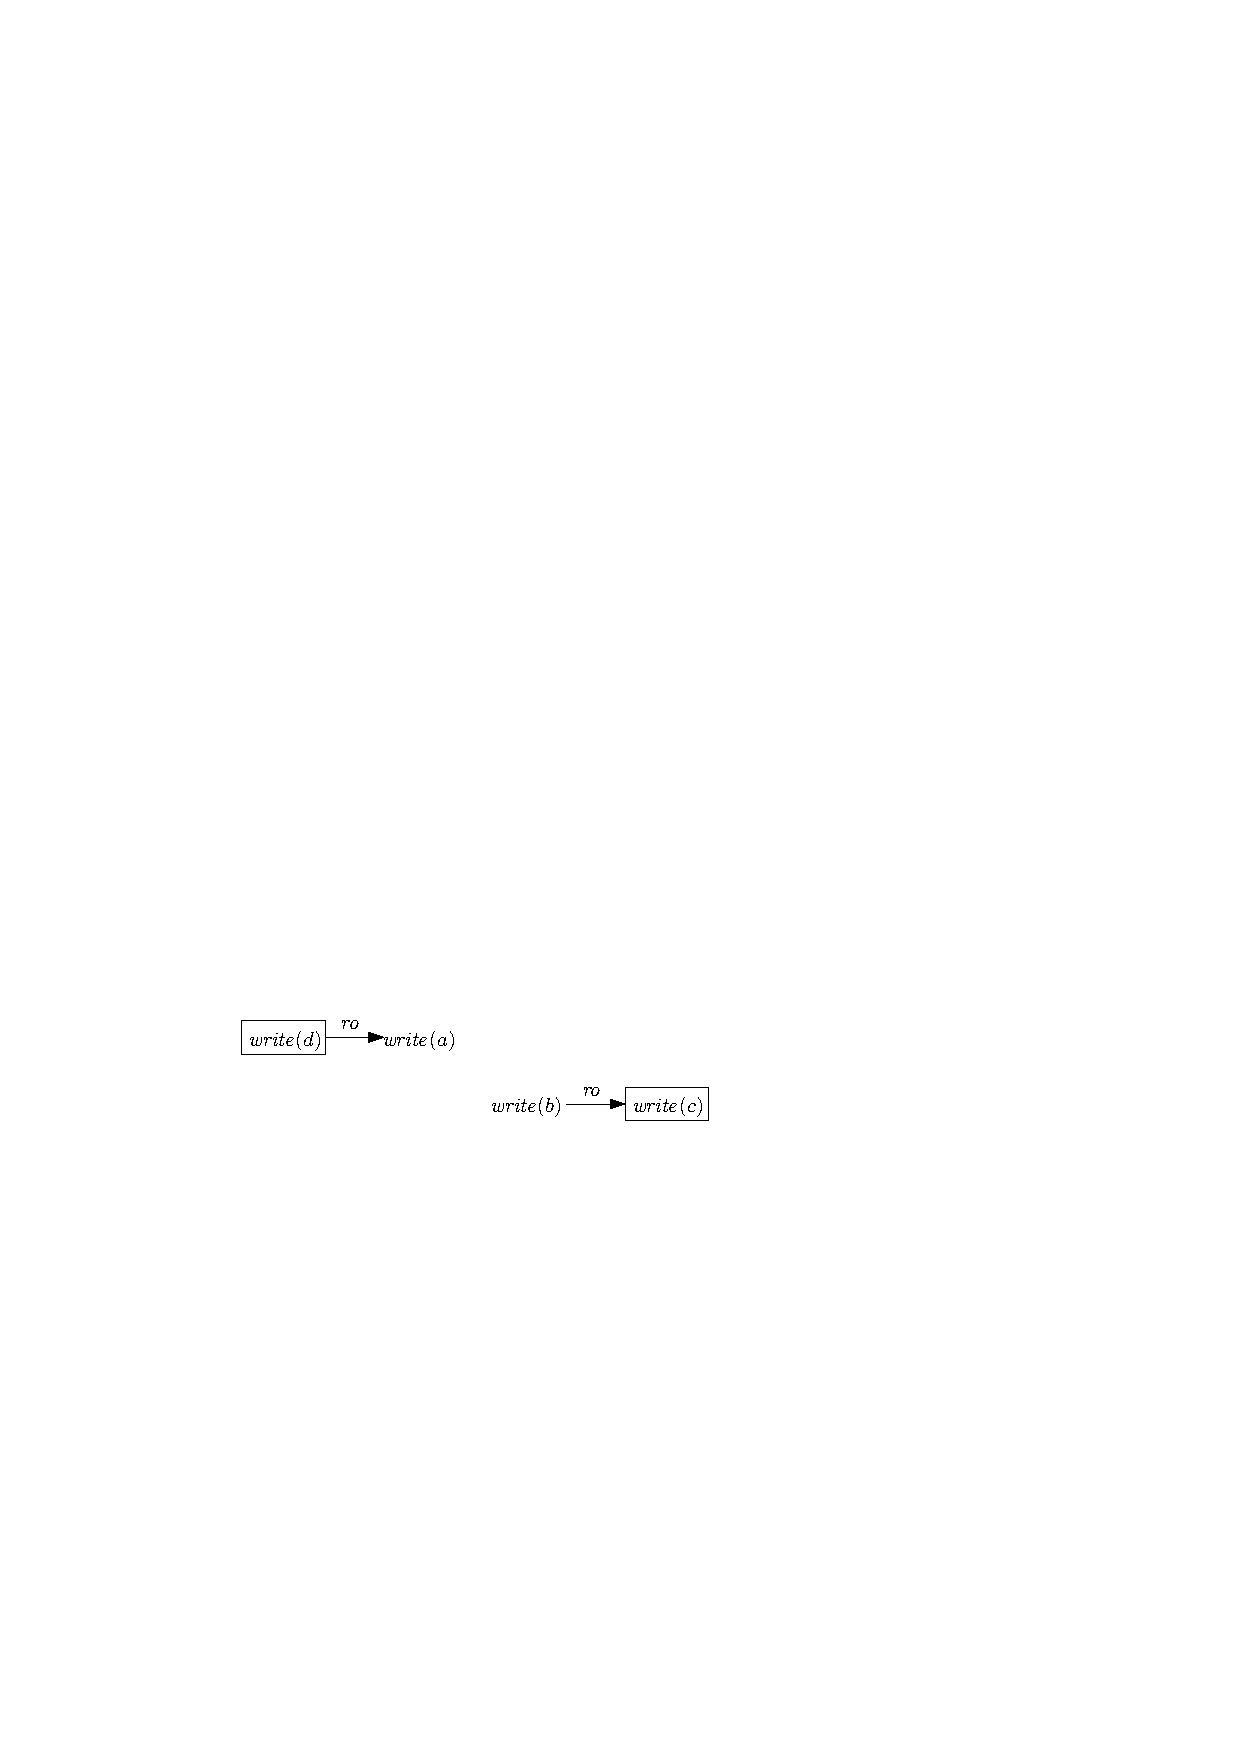
\includegraphics[width=0.35 \textwidth]{figures/TwoSubLin-NotaGlobalLin.pdf}
\vspace{-5pt}
  \caption{A history with two OR-Set objects showing that per-object \crdtlinearization{s} cannot be combined into a global \crdtlinearization{}. Every operation is delivered only to the origin replica and therefore, the visibility relation is defined by the horizontal lines (read from left to right).}
  \vspace{-5pt}
  \label{fig:negative_composition}
\end{wrapfigure}

The standard notion of linearizability~\cite{HerlihyW90} ensures that the composition of a set of linearizable objects is also linearizable. More precisely, it ensures that for every history, any per-object linearizations, concerning the operations of a single object, can be combined into a global linearization, concerning all the operations in the history. By combining linearizations, we mean constructing a global linearization whose projections on the operations of a single object are exactly the per-object linearizations considered in the beginning.
However, this is not true for our notion of RA-linearizability. An example of a history showing this fact is given in \figureautorefname~\ref{fig:negative_composition}. This history contains operations of two OR-Set objects $\aobj_1$ and $\aobj_2$, the operations of $\aobj_1$ being represented using blank circles and the operations of $\aobj_2$ using filled circles. The operations of $\aobj_1$ can be linearized to $\aobj_1.\alabelshort[{\tt add}]{c}\cdot \aobj_1.\alabelshort[{\tt add}]{d}$ (this is a valid \crdtlinearization{} since any sequence of ${\tt add}$ operations is admitted by $\specOrSet$) while the operations of $\aobj_2$ can be linearized to $\aobj_2.\alabelshort[{\tt add}]{a}\cdot \aobj_2.\alabelshort[{\tt add}]{b}$. There is no \crdtlinearization{} of this history whose projections on each of the two objects correspond to these per-object linearizations: trying to construct a linearization where $\aobj_2.\alabelshort[{\tt add}]{a}$ occurs before $\aobj_2.\alabelshort[{\tt add}]{b}$ will imply that $\aobj_1.\alabelshort[{\tt add}]{d}$ must occur before $\aobj_1.\alabelshort[{\tt add}]{c}$ (since it must be consistent with the visibility relation), which contradicts the linearization of $\aobj_1$, and similarly for the other case, when trying to construct a global linearization consistent with the linearization of $\aobj_2$'s operations. A reader knowledgeable of the literature on linearizability may notice that this discrepancy between standard linearizability and RA-linearizability comes from the fact that the partial order defining a history in the case of standard linearizability is actually an interval order~\footnote{A partial order $R$ is an interval-order if $\{(a,b), (c,d)\} \subseteq R$ implies that $(a,d) \in R$ or $(c,b) \in R$, for every $a,b,c,d$.}, while in the case of RA-linearizability it is an arbitrary partial order.
%\gpwarning[nomargin, inline]{I think this would be a place to talk about~\cite{JagadeesanR18}.}


\subsection{Composing Objects That Admit Execution-Order Linearizations}


Although not all per-object \crdtlinearization{s} can be combined into global \crdtlinearization{s}, this may still be true in some cases. For instance, let us consider again the history in \autoref{fig:negative_composition}. The operations of $\aobj_1$ can also be linearized to $\aobj_1.\alabelshort[{\tt add}]{d}\cdot \aobj_1.\alabelshort[{\tt add}]{c}$ which enables a global \crdtlinearization{} $\aobj_1.\alabelshort[{\tt add}]{d}\cdot \aobj_2.\alabelshort[{\tt add}]{a}\cdot \aobj_2.\alabelshort[{\tt add}]{b}\cdot \aobj_1.\alabelshort[{\tt add}]{c}$ whose projection on individual objects is consistent with the per-object linearizations (we consider the same linearization $\aobj_2.\alabelshort[{\tt add}]{a}\cdot \aobj_2.\alabelshort[{\tt add}]{b}$ for $\aobj_2$).

We show that in the case of \crdtlinearizable{} objects that admit execution-order linearizations, there always exist per-object \crdtlinearization{s} that can be combined into global \crdtlinearization{s}, which implies that their composition is \crdtlinearizable{}. Moreover, their composition also admits execution-order linearizations. A first preliminary result states that the order in which concurrent operations are executed at the origin replica can be permuted arbitrarily while still leading to a valid trace. More precisely, for every linearization $\alinord$ of the visibility in the history of a trace, there exists another valid trace where operations are executed at the origin replica in the order defined by $\alinord$.

\begin{lemma}\label{lem:trace_closure}
Let $\atrace$ be a trace of an object $\aobj$ and $\hist{\atrace}=(\alabelset,\avisord)$. Then, for every sequence $(\alabelset,\alinord)$ which is consistent with $\avisord$ (i.e., $\avisord
    \cup \alinord$ is acyclic), there exists a trace $\atrace'$ of $\aobj$ such that $\src{}{\alabel_1}$ occurs before $\src{}{\alabel_2}$ in $\atrace'$ iff $\alabel_1$ occurs before $\alabel_2$ in $\alinord$. Moreover, $\atrace'$ has the same history as $\atrace$.
\end{lemma}
\begin{proof}(Skech)
We define a \emph{dependency} relation $\circledcirc$ between actions as follows: $\src{\arep_1}{\alabel_1}\circledcirc \dwn{\arep_2}{\alabel_2}$ iff $\arep_1=\arep_2$ or $\alabel_1=\alabel_2$, $\src{\arep_1}{\alabel_1}\circledcirc \src{\arep_2}{\alabel_2}$ iff $\arep_1=\arep_2$, $\dwn{\arep_1}{\alabel_1}\circledcirc \src{\arep_2}{\alabel_2}$ iff $\arep_1=\arep_2$, and $\dwn{\arep_1}{\alabel_1}\circledcirc \dwn{\arep_2}{\alabel_2}$ iff $\arep_1=\arep_2$. Given a trace $\atrace=\atrace_1\cdot \aact_1\cdot\aact_2\cdot\atrace_2$, we say that a trace $\atrace'=\atrace_1\cdot \aact_2\cdot\aact_1\cdot\atrace_2$ is derived from $\atrace$ by a \emph{$\circledcirc$-valid swap} iff $\aact_1$ and $\aact_2$ are \emph{not} related by $\circledcirc$. Using standard reasoning about traces of a concurrent system, it can be shown that if $\atrace$ is a trace of $\aobj$, then any trace $\atrace'$ derived through a sequence of $\circledcirc$-valid swaps is also a trace of $\aobj$. Moreover, $\atrace'$ has the same history as $\atrace$. Then, by the definition of the visibility relation $\avisord$ in the history of a trace and the causal delivery assumption, it can be shown that given a trace $\atrace$ of $\aobj$ containing two actions $\src{}{\alabel_1}$ and $\src{}{\alabel_2}$ such that $\alabel_1$ and $\alabel_2$ are concurrent and $\src{}{\alabel_1}$ occurs before $\src{}{\alabel_2}$, there exists another trace $\atrace'$ of $\aobj$ that is defined through a sequence of $\circledcirc$-valid swaps and where $\src{}{\alabel_2}$ occurs before $\src{}{\alabel_1}$. Therefore, the order in which generator actions of concurrent operations occur in a trace can be permuted arbitrarily, which implies the claim of the lemma.
\end{proof}

Lemma~\ref{lem:trace_closure} implies that given an \crdtlinearizable{} object $\aobj$, if it admits execution-order linearizations, then every linearization of a history of $\aobj$ consistent with visibility is a valid \crdtlinearization{}.

\begin{lemma}\label{lem:t0_lin}
Let $\aobj$ be an object which is \crdtlinearizable{} w.r.t. a specification $\Spec$ and admits execution-order linearizations. Then, for every history $\ahist=(\alabelset,\avisord)$ of $\aobj$ and every sequence $(\alabelset,\alinord)$ which is consistent with $\avisord$, we have that $(\alabelset,\alinord)$ is an \crdtlinearization{} of $\ahist$ w.r.t. $\Spec$.
\end{lemma}
\begin{proof}(Skech)
Let $(\alabelset,\alinord)$ be a sequence consistent with the visibility relation of $\ahist$. By Lemma~\ref{lem:trace_closure}, there exists a trace $\atrace$ of $\aobj$ such that  $\src{}{\alabel_1}$ occurs before $\src{}{\alabel_2}$ in $\atrace$ iff $\alabel_1$ occurs before $\alabel_2$ in $\alinord$. Definition~\ref{def:exec_order} implies that $(\alabelset,\alinord)$ is an RA-linearization of $\hist{\atrace}=\ahist$.
\end{proof}

Lemma~\ref{lem:t0_lin} is the essential ingredient for proving that the composition of a set of \crdtlinearizable{} objects that admit execution-order linearizations is also \crdtlinearizable{}. Intuitively, given a history $\ahist$ with multiple such objects, any linearization of $\ahist$ is a valid \crdtlinearization{} since each of its projections on the set of operations of a single object is a linearization of the per-object visibility relation~\footnote{By definition, the visibility relation in the history of an object composition $\aobj_1\comp\aobj_2$ projected on operations of $\aobj_1$, resp., $\aobj_2$, is exactly the visibility relation stored in the global configurations of $\aobj_1$, resp., $\aobj_2$ (at the end of the execution that produces that history).}  and thus, a valid \crdtlinearization{} of that object.

\begin{theorem}\label{th:comp_execution_order}
The composition of a set of \crdtlinearizable{} objects that admit execution-order linearizations is \crdtlinearizable{}. Moreover, the composition admits execution-order linearizations.
\end{theorem}
%\begin{proof}(Skech)
%TODO
%\end{proof}

%\begin{definition}[\tzerolin{}]
%\label{definition:t0-linearizability}
%A single-object history $\ahis$ is \tzerolinearizable{} w.r.t a sequential specification \Spec{}, if $\ahis$ is \crdtlinearizable{} w.r.t \Spec{}, and each specification sequence $(\alabelset, \aseqord)$ consistent with visibility order is a \crdtlinearization{}.
%\end{definition}

\subsection{Composing Objects That Admit Timestamp-Order Linearizations}

%We say a specification sequence $(\alabelset, \aseqord)$ be consistent with timestamp order, if the time-stamp of operation $\aobj_1$ being less than the timestamp of $\aobj_2$ implies that $\aobj_1$ being before $\aobj_2$ in $\aseqord$, and if $(\aobj_3,\aobj_4) \in \avisord$, then the timestamp of $\aobj_3$ is less or equal to the timestamp of $\aobj_4$.
%
%\begin{definition}[\tonelin{}]
%\label{definition:t1-linearizability}
%A single-object history $\ahis$ is \tonelinearizable{} w.r.t a sequential specification \Spec{}, if $\ahis$ is \crdtlinearizable{} w.r.t \Spec{}, and each specification sequence $(\alabelset, \aseqord)$ consistent with visibility order and timestamp order is a \crdtlinearization{}.
%\end{definition}

\begin{figure}[t]
  \centering
  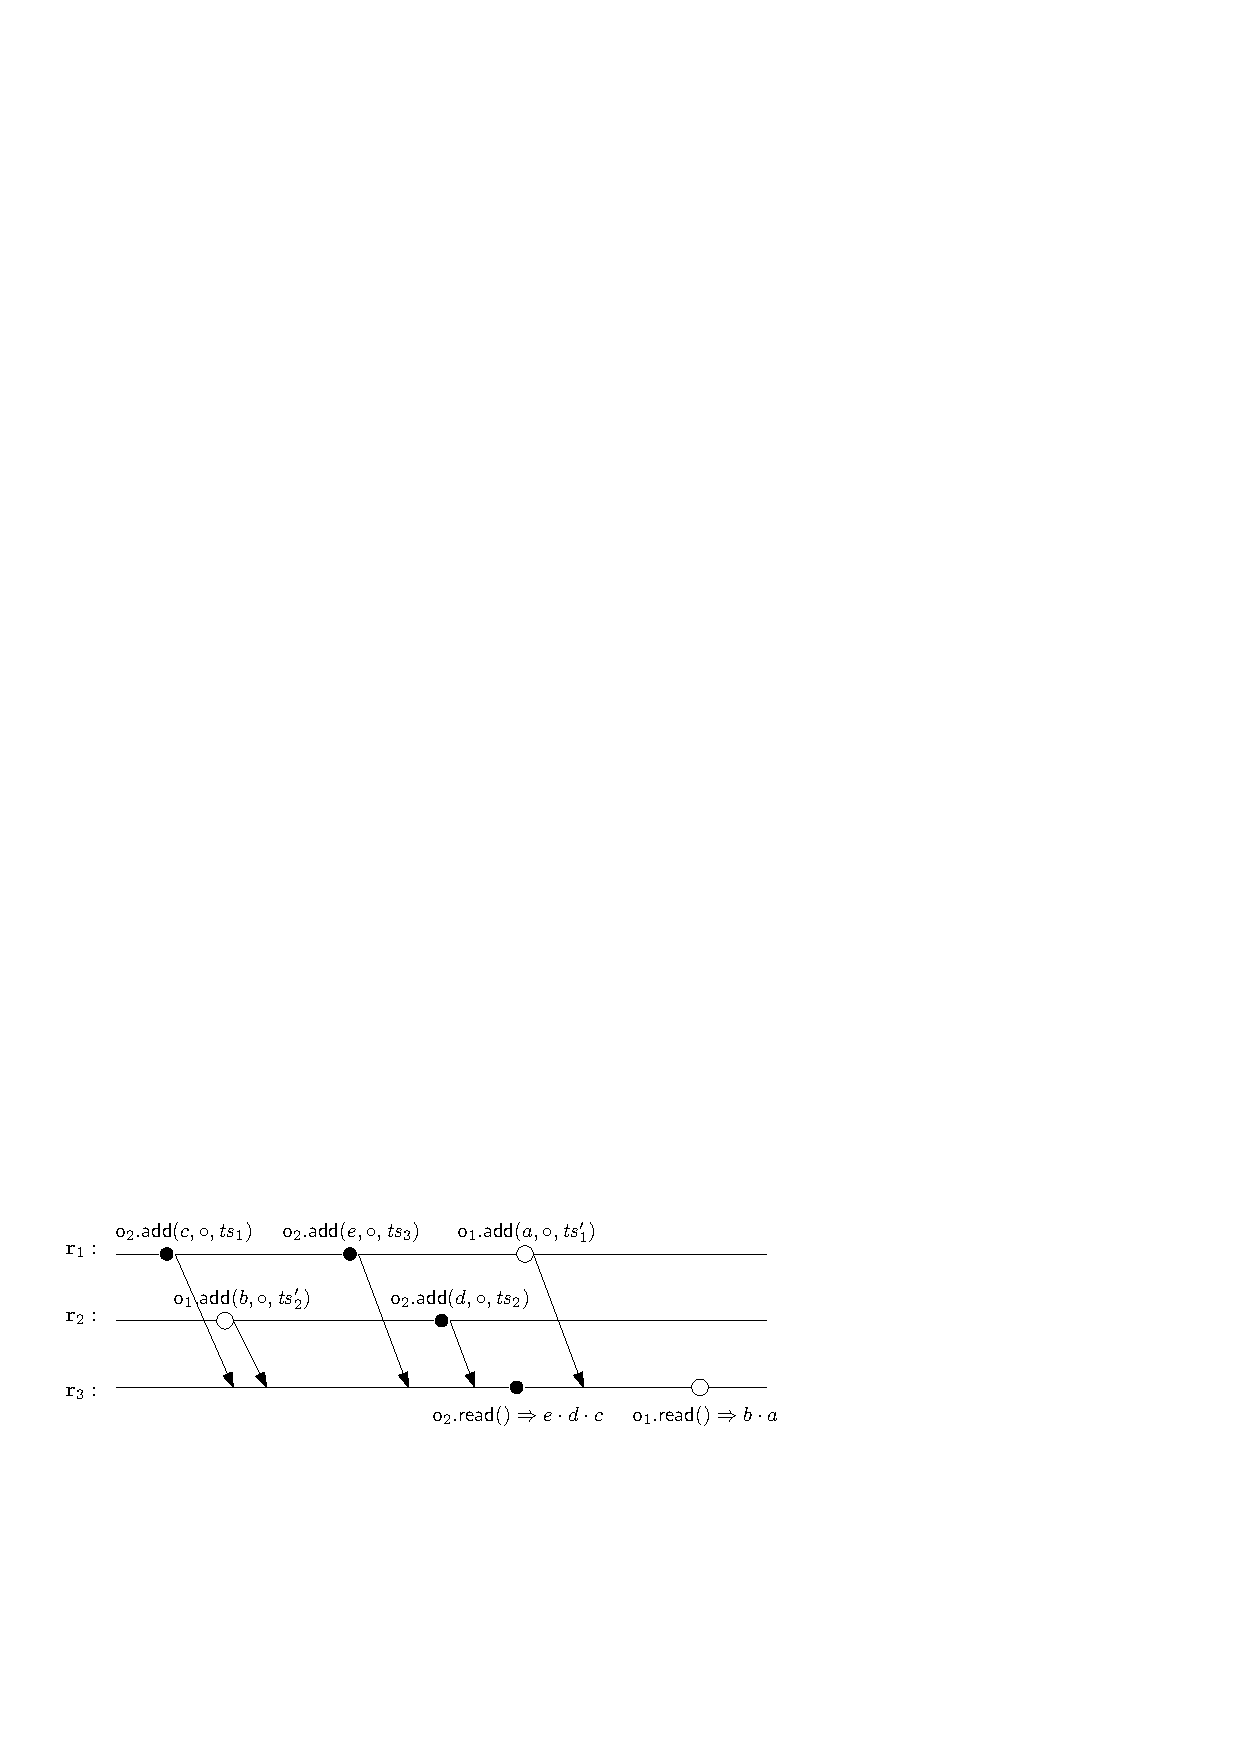
\includegraphics[width=0.7 \textwidth]{figures/LWWReg-LWWReg-NoSTS.pdf}
%\vspace{-10pt}
  \caption{A history showing that the composition $\otimes$ of two RGA objects is not \crdtlinearizable{}.}
  \label{fig:negative_ts_composition}
\end{figure}


The positive result in Theorem~\ref{th:comp_execution_order} does not apply directly to objects that admit timestamp-order linearizations. The main reason is that the unrestricted object composition $\otimes$ defined in \sectionautorefname~\ref{ssec:comp_intro} allows different objects to generate timestamps independently, and in ``conflicting'' orders along some execution. For instance, \figureautorefname~\ref{fig:negative_ts_composition} shows a history with two RGA objects $\aobj_1$ and $\aobj_2$. We assume that $\ats_1 < \ats_2 < \ats_3$ and $\ats'_1 < \ats'_2$ (the orderings between unprimed and primed timestamps are not important). The operations of $\aobj_1$ can be linearized to
\begin{align*}
\aobj_1.\alabelshort[{\tt addAfter}]{\circ,a}\cdot \aobj_1.\alabelshort[{\tt addAfter}]{\circ,b}\cdot \aobj_1.\alabellongind[{\tt read}]{}{b\cdot a}{}
\end{align*}
and the operations of $\aobj_2$ to
\begin{align*}
\aobj_2.\alabelshort[{\tt addAfter}]{\circ,c}\cdot \aobj_2.\alabelshort[{\tt addAfter}]{\circ,d}\cdot \aobj_2.\alabelshort[{\tt addAfter}]{\circ,e}\cdot \aobj_2.\alabellongind[{\tt read}]{}{e\cdot d\cdot c}{}
\end{align*}
Note that these are the only \crdtlinearization{s} possible for these operations. It can be easily seen that there is no ``global'' linearization consistent with these per-object linearizations. Ordering $\alabelshort[{\tt addAfter}]{\circ,a}$ before $\alabelshort[{\tt addAfter}]{\circ,b}$ implies that $\alabelshort[{\tt addAfter}]{\circ,e}$ should occur before $\alabelshort[{\tt addAfter}]{\circ,d}$ which contradicts the second linearization above.
We solve this problem by requiring an additional constraint on the composition operator $\comp$ such that intuitively, all objects use a common timestamp generator. This in turn requires that the implementation of the objects share a common timestamp generator, and it must ensure that each new timestamp is bigger than the  timestamps used by operations delivered to a replica, independently of the object on which they are applied. For instance, the history of \figureautorefname~\ref{fig:negative_ts_composition} would not be admitted because $\ats_1'$ should be bigger than $\ats_3$ (since the operation that received $\ats_3$ from the timestamp generator originates from the same replica as the operation receiving $\ats_1'$ at a later time) and $\ats_2$ should be bigger than $\ats_2'$. These two constraints together with $\ats_1'<\ats_2'$ contradict the fact that $\ats_2 < \ats_3$.
%
We remark here that while this requires a modification of the algorithms, where the timestamp generator is a parameter, this has no algorithmic of run-time cost, and in fact a similar idea have been suggested in the systems literature (e.g.~\cite{EnesPB17}).

%Before going into the details of our solution, we present a formal definition of timestamp-order linearizations. For a history $\ahist=(\alabelset,\avisord)$, we define the timestamp $\tsof_\ahist(\alabel)$ of a label $\alabel$ in the context of the history $h$ to be $\tsof_\ahist(\alabel)=\tsof(\alabel)$ if $\tsof(\alabel)\neq\bot$ and $\tsof_\ahist(\alabel)=\mathsf{max}\, \{\tsof(\alabel'):(\alabel',\alabel)\in \avisord \}$, otherwise.
%
%\begin{definition}
%An object $\aobj$ which is \crdtlinearizable{} w.r.t. a specification $\Spec$ admits \emph{timestamp-order linearizations} if for every trace $\atrace\in\traces(\aobj)$ with $\hist{\atrace}=(\alabelset,\avisord)$, there exists an \crdtlinearization{} $(\alabelset,\alinord)$ of $\hist{\atrace}$ w.r.t. $\Spec$ such that $\alabel_1$ occurs before $\alabel_2$ in $\alinord$ iff $\tsof_\ahist(\alabel_1) < \tsof_\ahist(\alabel_2)$ or $\src{}{\alabel_1}$ occurs before $\src{}{\alabel_2}$ in $\atrace$, for every two labels $\alabel_1,\alabel_2\in\alabelset$.
%\end{definition}

Using again Lemma~\ref{lem:trace_closure}, which ensures that the generators of ``concurrent'' operations can be executed in any order, we get that for any \crdtlinearizable{} object $\aobj$ which admits timestamp-order linearizations, every linearization of a history of $\aobj$ which is also consistent with the order between timestamps is a valid \crdtlinearization{}.
For a history $\ahist=(\alabelset,\avisord)$, let $\atsord{\ahist}$ be an order between the labels in $\alabelset$ such that $\alabel_1\atsord{\ahist}\alabel_2$ iff $\tsof_\ahist(\alabel_1) < \tsof_\ahist(\alabel_2)$.

\begin{lemma}
Let $\aobj$ be an object which is \crdtlinearizable{} w.r.t. a specification $\Spec$ and admits timestamp-order linearizations. Then, for every history $\ahist=(\alabelset,\avisord)$ of $\aobj$ and every sequence $(\alabelset,\alinord)$ which is consistent with $\avisord$ and $\atsord{\ahist}$, we have that $(\alabelset,\alinord)$ is an \crdtlinearization{} of $\ahist$ w.r.t. $\Spec$.
\end{lemma}

\begin{figure}[t]
  \centering
  \footnotesize
\[
  \inferrule[\text{\sc Operation}]
  {\alabel = \aobj_k.\alabellongind{\argv}{\retv}{(i,\ats)}\mbox{ with } k\in \{1,2\} \\ (\gstates_k, \avisord_k, \downstreams_k) \xrightarrow{\src{\arep}{\alabel}}_{k} (\gstates_k', \avisord_k', \downstreams_k') \\
  (\gstates'_{k'}, \avisord'_{k'}, \downstreams'_{k'}) = (\gstates_{k'}, \avisord_{k'}, \downstreams_{k'})\mbox{ for $k'\neq k$} \\
  \gstates_1(\arep) = (\alabelset_1, \astate_1) \\ \gstates_2(\arep) = (\alabelset_2, \astate_2) \\
  \ats\neq\bot\implies (\,\forall \alabel\in\alabelset_1\cup\alabelset_2.\ \tsof(\alabel)\neq\bot \implies \tsof(\alabel) < \ats\,) }
  {((\gstates_1, \avisord_1, \downstreams_1),(\gstates_2, \avisord_2, \downstreams_2)) \xrightarrow{\src{\arep}{\alabel}} (\gstates_1', \avisord_1', \downstreams_1'),(\gstates_2', \avisord_2', \downstreams_2')}
\]
\caption{The transition rule for generators in the object composition operator $\otimes_{\tsof}$.}
  \label{fig:comp-ts}
\end{figure}

We define a restriction $\otimes_{\tsof}$ of the object composition operator $\otimes$ such that the set of histories $h=(\alabelset,\avisord)$ in the composition $\aobj_1\otimes_{\tsof}\aobj_2$ satisfy the property that the order between timestamps (of all objects) is consistent with the visibility relation $\avisord$ (i.e., $\avisord\cup \atsord{\ahist}$ is acyclic). With respect to the ``unrestricted'' composition $\otimes$ defined in \sectionautorefname~\ref{ssec:comp_intro}, we only modify the transition rule corresponding to generators, as shown in \figureautorefname~\ref{fig:comp-ts}. The only addition consists in ensuring that when a new timestamp is generated, it is bigger than all the timestamps ``visible'' to the replica executing that generator (even if they were generated in the context of a different object). Its extension to a set of objects is defined as usual. The composition operator  $\otimes_{\tsof}$ is called \emph{shared timestamp generator composition}. From a practical point of view, if we were to consider the standard timestamp mechanism used in CRDTs, i.e., each replica maintains a counter which is increased monotonically with every new operation (originating at the replica or delivered from another replica) and timestamps are defined as pairs of replica identifiers and counter values, then $\otimes_{\tsof}$ can be implemented using a ``shared'' counter which increases monotonically with every new operation, independently of the object on which it is applied.

The following theorem shows that composing \crdtlinearizable{} objects that admit execution-order or timestamp-order linearizations, i.e., they can be proved \crdtlinearizable{} using the methodologies described in \sectionautorefname~\ref{subsec:time order of execution as linearization} and \sectionautorefname~\ref{subsec:time-stamp order as linearizabtion}, is \crdtlinearizable{}, provided that all the objects share the same timestamp generator.

\begin{theorem}\label{th:comp_all}
The shared timestamp generator composition of a set of \crdtlinearizable{} objects that admit execution-order or timestamp-order linearizations is \crdtlinearizable{}.
\end{theorem}
%\begin{proof}(Sketch)
%TODO
%\end{proof}

Based on the results in Theorem~\ref{th:execution_order_objects} and Theorem~\ref{th:ts_order_objects}, the theorem above shows that any shared timestamp generator composition of the objects mentioned in \figureautorefname~\ref{fig:crdt-implementaton of this paper, their correctness, and their interface} is RA-linearizable.

% 
\subsection{Tables and Graphs}
\label{lemma:tables and graphs}

{\color {red}CW: I put some tables and graphs here.}

{\color {red}CW: We should make agreement about the interface.}

\figurename~\ref{fig:crdt-implementaton of this paper, their correctness, and their interface} gives the \crdtimp{} proved in our work, their correctness, and their interface (methods).

% \begin{figure}[t]
% %\centering

% \begin{tabular}{|l|c|r|}
% \hline
% \crdtimp&Correctness&Interface\\
% \hline
% counter~\cite{ShapiroPBZ11}&\tzerolin&$\alabelshort[{\tt inc}]{}$, $\alabelshort[{\tt dec}]{}$\\
% \hline
% PN-counter~\cite{ShapiroPBZ11}&\tzerolin&$\alabelshort[{\tt inc}]{}$, $\alabelshort[{\tt dec}]{}$\\
% \hline
% LWW-register~\cite{DBLP:journals/rfc/rfc677}&\tonelin&$\alabelshort[{\tt write}]{value}$, $\alabellong[{\tt read}]{}{value}{}$\\
% \hline
% Multi-value register~\cite{DBLP:conf/sosp/DeCandiaHJKLPSVV07}&\tzerolin&$\alabelshort[{\tt write}]{value}$, $\alabellong[{\tt read}]{}{Set \ value}{}$\\
% \hline
% 2P-set~\cite{ShapiroPBZ11}&\tzerolin&$\alabelshort[{\tt add}]{value}$, $\alabelshort[{\tt remove}]{value}$, $\alabellong[{\tt read}]{}{Set \ value}{}$\\
% \hline
% LWW-set~\cite{ShapiroPBZ11}&\tonelin&$\alabelshort[{\tt add}]{value}$, $\alabelshort[{\tt remove}]{value}$, $\alabellong[{\tt read}]{}{Set \ value}{}$\\
% \hline
% %PN-set~\cite{ShapiroPBZ11}&not \crdtlinearizable{}&$add$, $remove$, $read$\\
% %\hline
% OR-set~\cite{ShapiroPBZ11}&\tzerolin&$\alabelshort[{\tt add}]{value}$, $\alabelshort[{\tt remove}]{value}$, $\alabellong[{\tt read}]{}{Set \ value}{}$\\
% \hline
% RGA~\cite{DBLP:journals/jpdc/RohJKL11}&\tonelin&$\alabelshort[{\tt addAfter}]{value,value}$, $\alabelshort[{\tt remove}]{value}$,
%                 \\ & & $\alabellong[{\tt read}]{}{List \ value}{}$\\
% \hline
% Wooki~\cite{DBLP:conf/wise/WeissUM07}&\tzerolin&$\alabelshort[{\tt addBetween}]{value,value,value}$, $\alabelshort[{\tt remove}]{value}$,
%                 \\ & & $\alabellong[{\tt read}]{}{List \ value}{}$\\
% \hline
% Treedoc~\cite{DBLP:conf/icdcs/PreguicaMSL09}&\tzerolin&$\alabelshort[{\tt addBetween}]{value,value,value}$, $\alabelshort[{\tt remove}]{value}$,
%                 \\ & & $\alabellong[{\tt read}]{}{List \ value}{}$\\
% \hline
% \end{tabular}

% \caption{\crdtimp{} of this paper, their correctness, and their interface.}
% \label{fig:crdt-implementaton of this paper, their correctness, and their interface}
% \end{figure}


% \figurename~\ref{fig:an example run of semantics} gives a example of two step of transitions on semantics of RGA. The first step is to do downstream of a $addAfter$, while the second step is to do operation $remove$. Here we can see that, the downstream of $addAfter$ always insert a new node into the Ti-tree $N$, while the downstream of $remove$ always insert a value into $Tomb$.

% \begin{figure}[t]
%   \centering
%   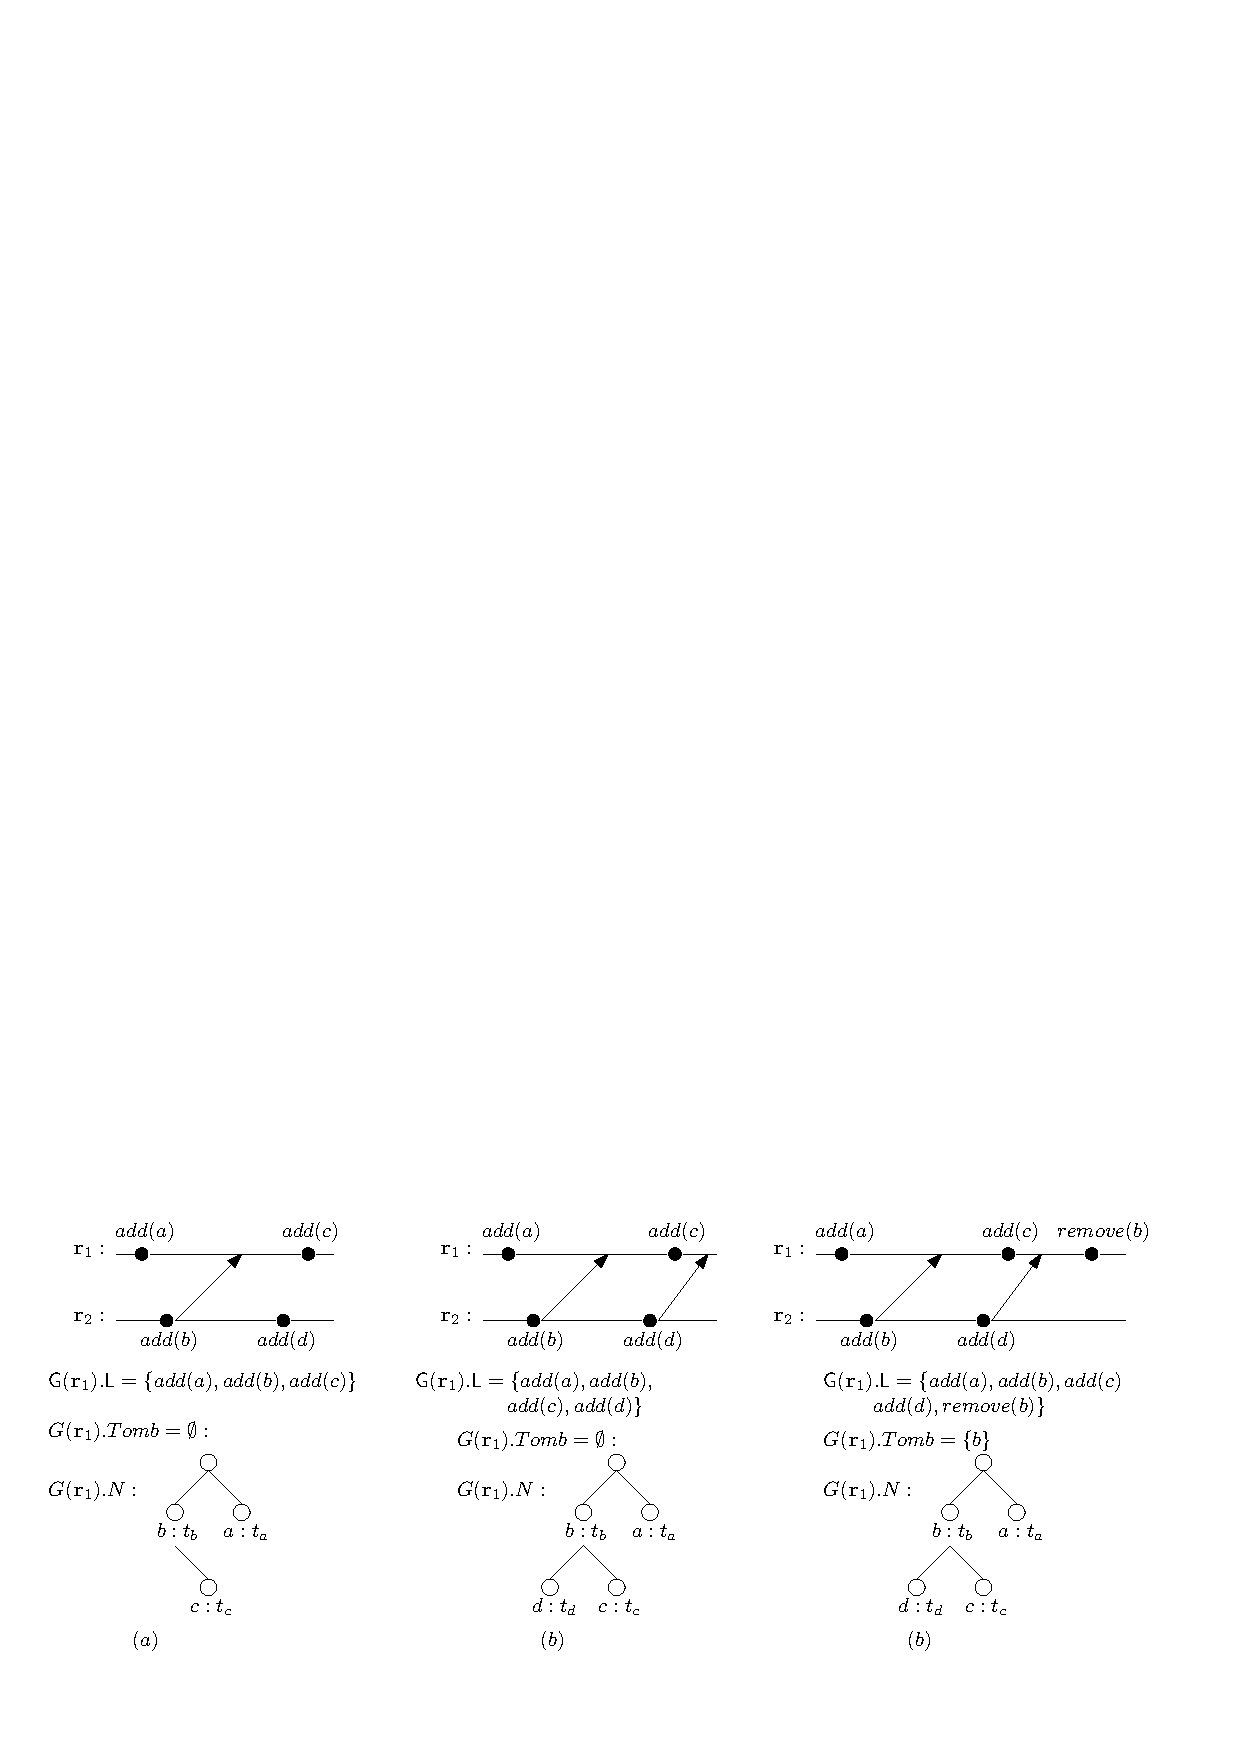
\includegraphics[width=1 \textwidth]{figures/ExplainSemantics.pdf}
% \vspace{-10pt}
%   \caption{An example run of semantics.}
%   \label{fig:an example run of semantics}
% \end{figure}


\figurename~\ref{fig:a history of RGA and its RA-linearization} gives a history of RGA and its \crdtlinearization{}.

\begin{figure}[t]
  \centering
  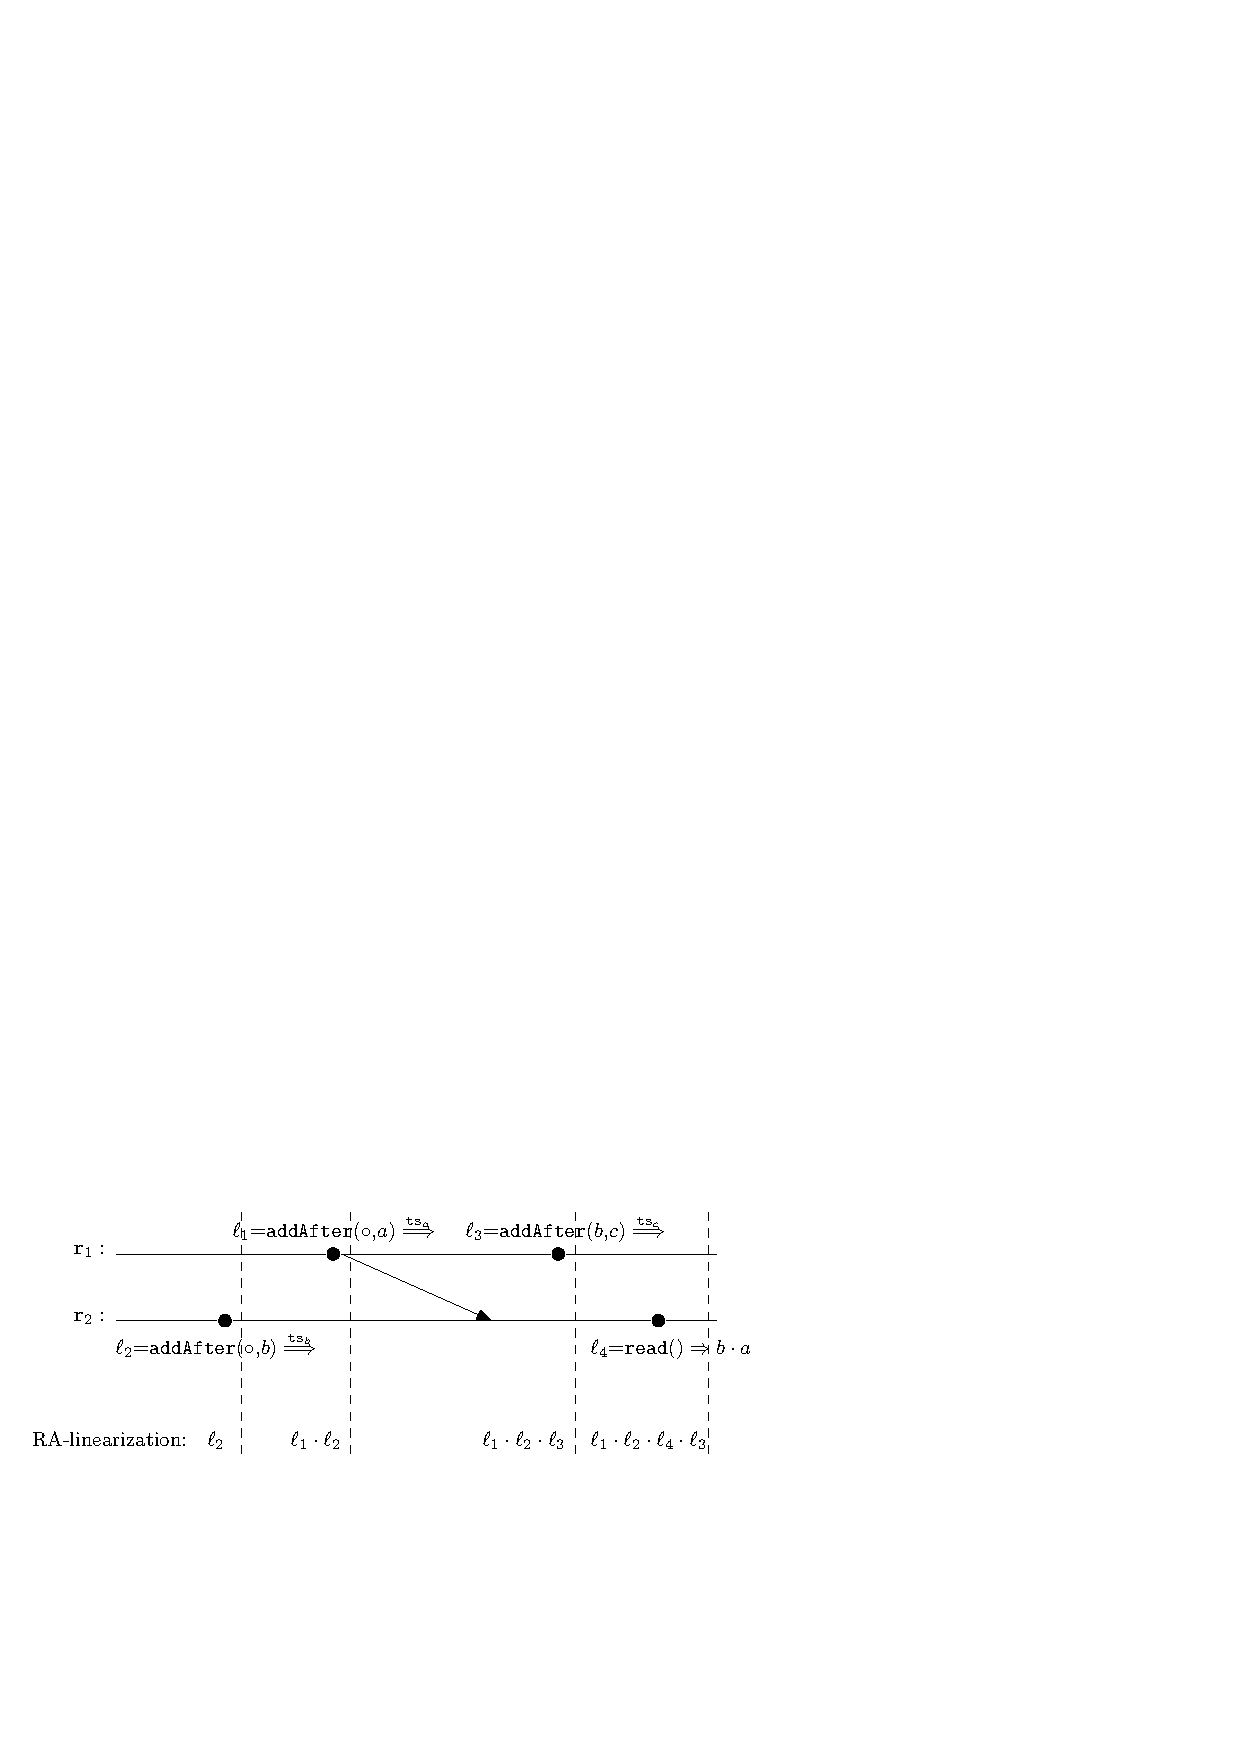
\includegraphics[width=0.6 \textwidth]{figures/RGAHisandLin.pdf}
\vspace{-10pt}
  \caption{A history of RGA and its \crdtlinearization{}.}
  \label{fig:a history of RGA and its RA-linearization}
\end{figure}


\figurename~\ref{fig:a history of OR-set, its update-query rewriting, and its RA-linearization} gives a history of OR-set, its query-update rewriting, and its \crdtlinearization{}.

\begin{figure}[t]
  \centering
  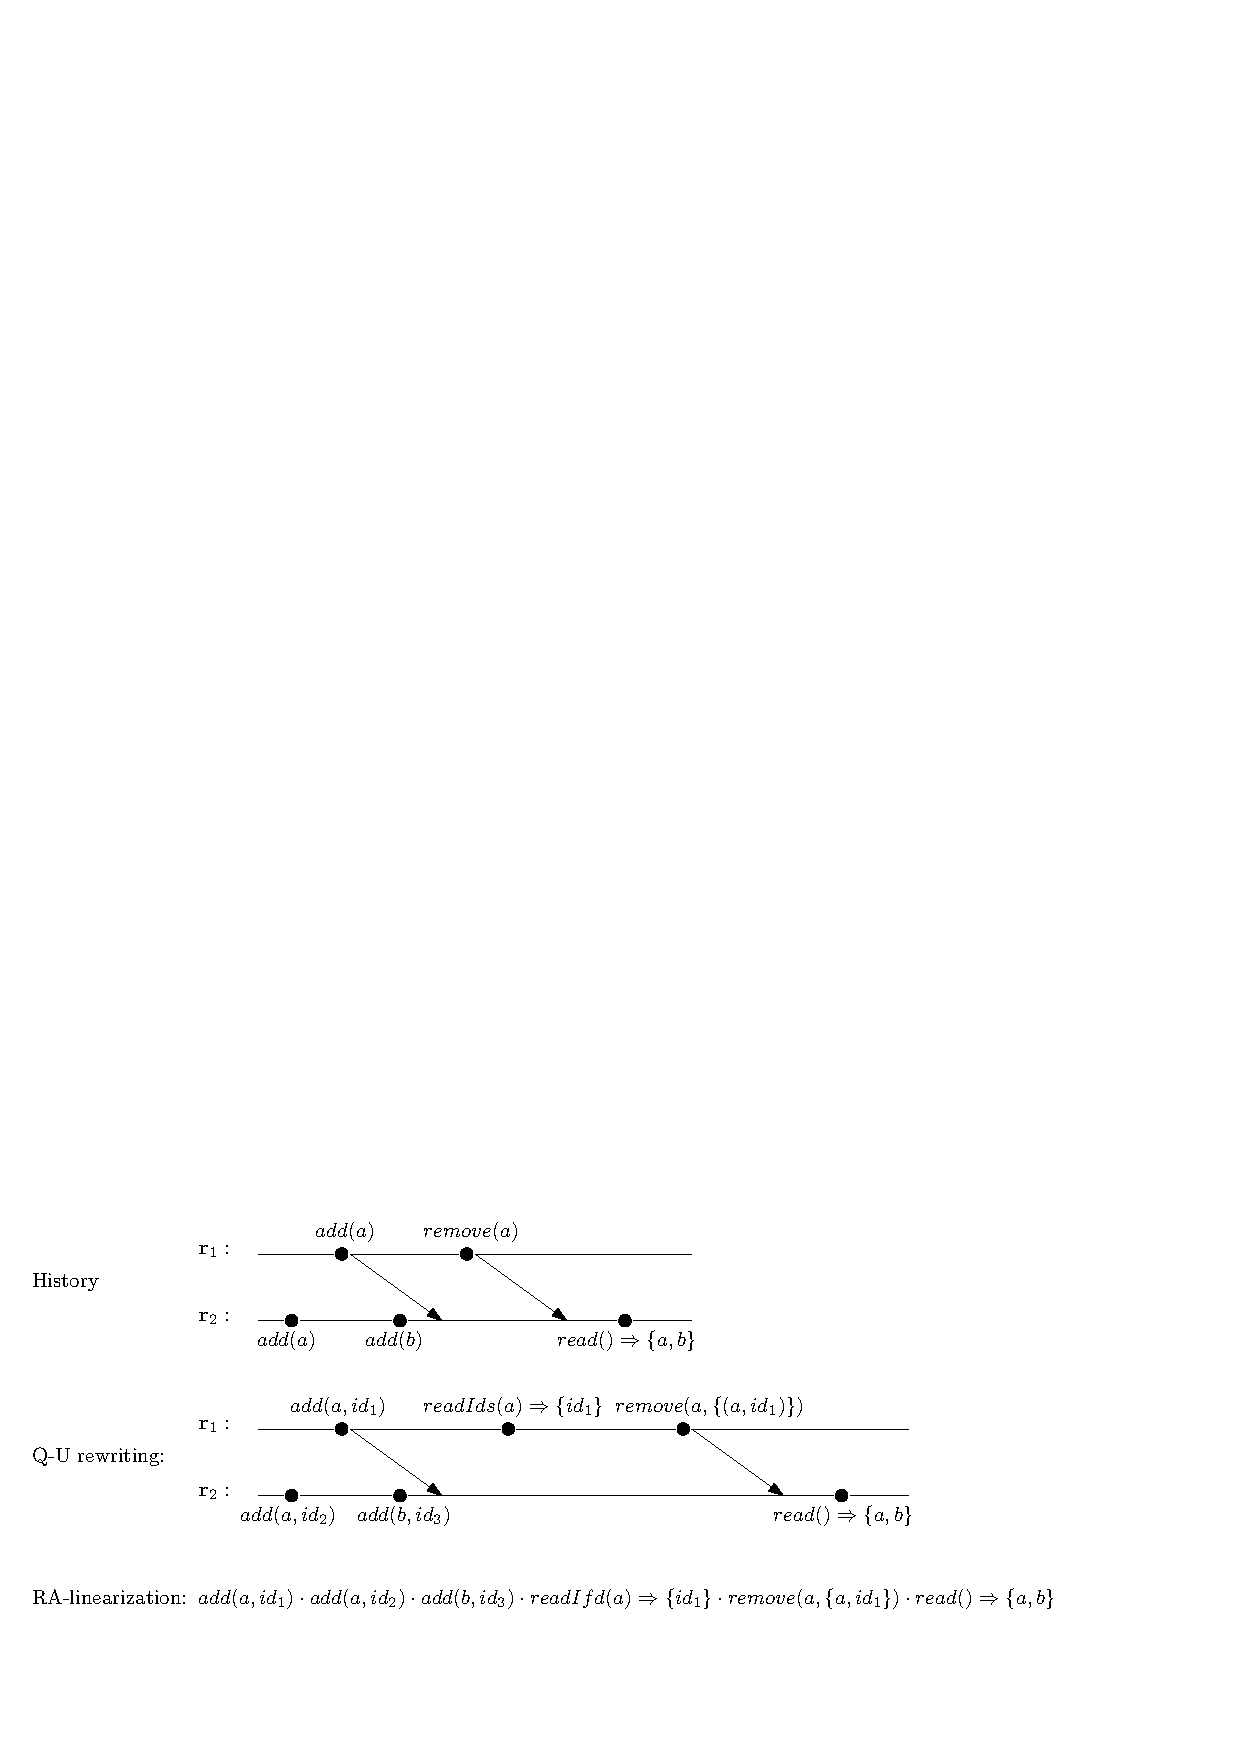
\includegraphics[width=0.8 \textwidth]{figures/ORSetHisRewritingandLin.pdf}
\vspace{-10pt}
  \caption{A history of OR-set, its update-query rewriting, and its \crdtlinearization{}.}
  \label{fig:a history of OR-set, its update-query rewriting, and its RA-linearization}
\end{figure}


\figurename~\ref{fig:how refinement mapping works} shows how refinement mapping works. \figurename~\ref{fig:how refinement mapping works} (a) shows the case of update labels, \figurename~\ref{fig:how refinement mapping works} (b) shows the case of query labels, and \figurename~\ref{fig:how refinement mapping works} (c) shows the case of update-query labels.

%Note that, in \figurename~\ref{fig:how refinement mapping works} (a) there is a ``gap'' between $\refmap(\sigma)$ and $\refmap(\sigma')$: it may be not the case that $\refmap(\sigma)\xRightarrow{\alabel}\refmap(\sigma')$. Although $\refmap(\sigma')$ should be obtained from $\refmap(\sigma_0)$ by a sequence of the same set of operations as from $\sigma_0$ to $\sigma'$, the order may be different. Such a transition exists for execution-order linearizations, and may not exist for timestamp-order linearizations. What we require here is only that the existence of $\refmap(\sigma')$.

\begin{figure}[t]
  \centering
  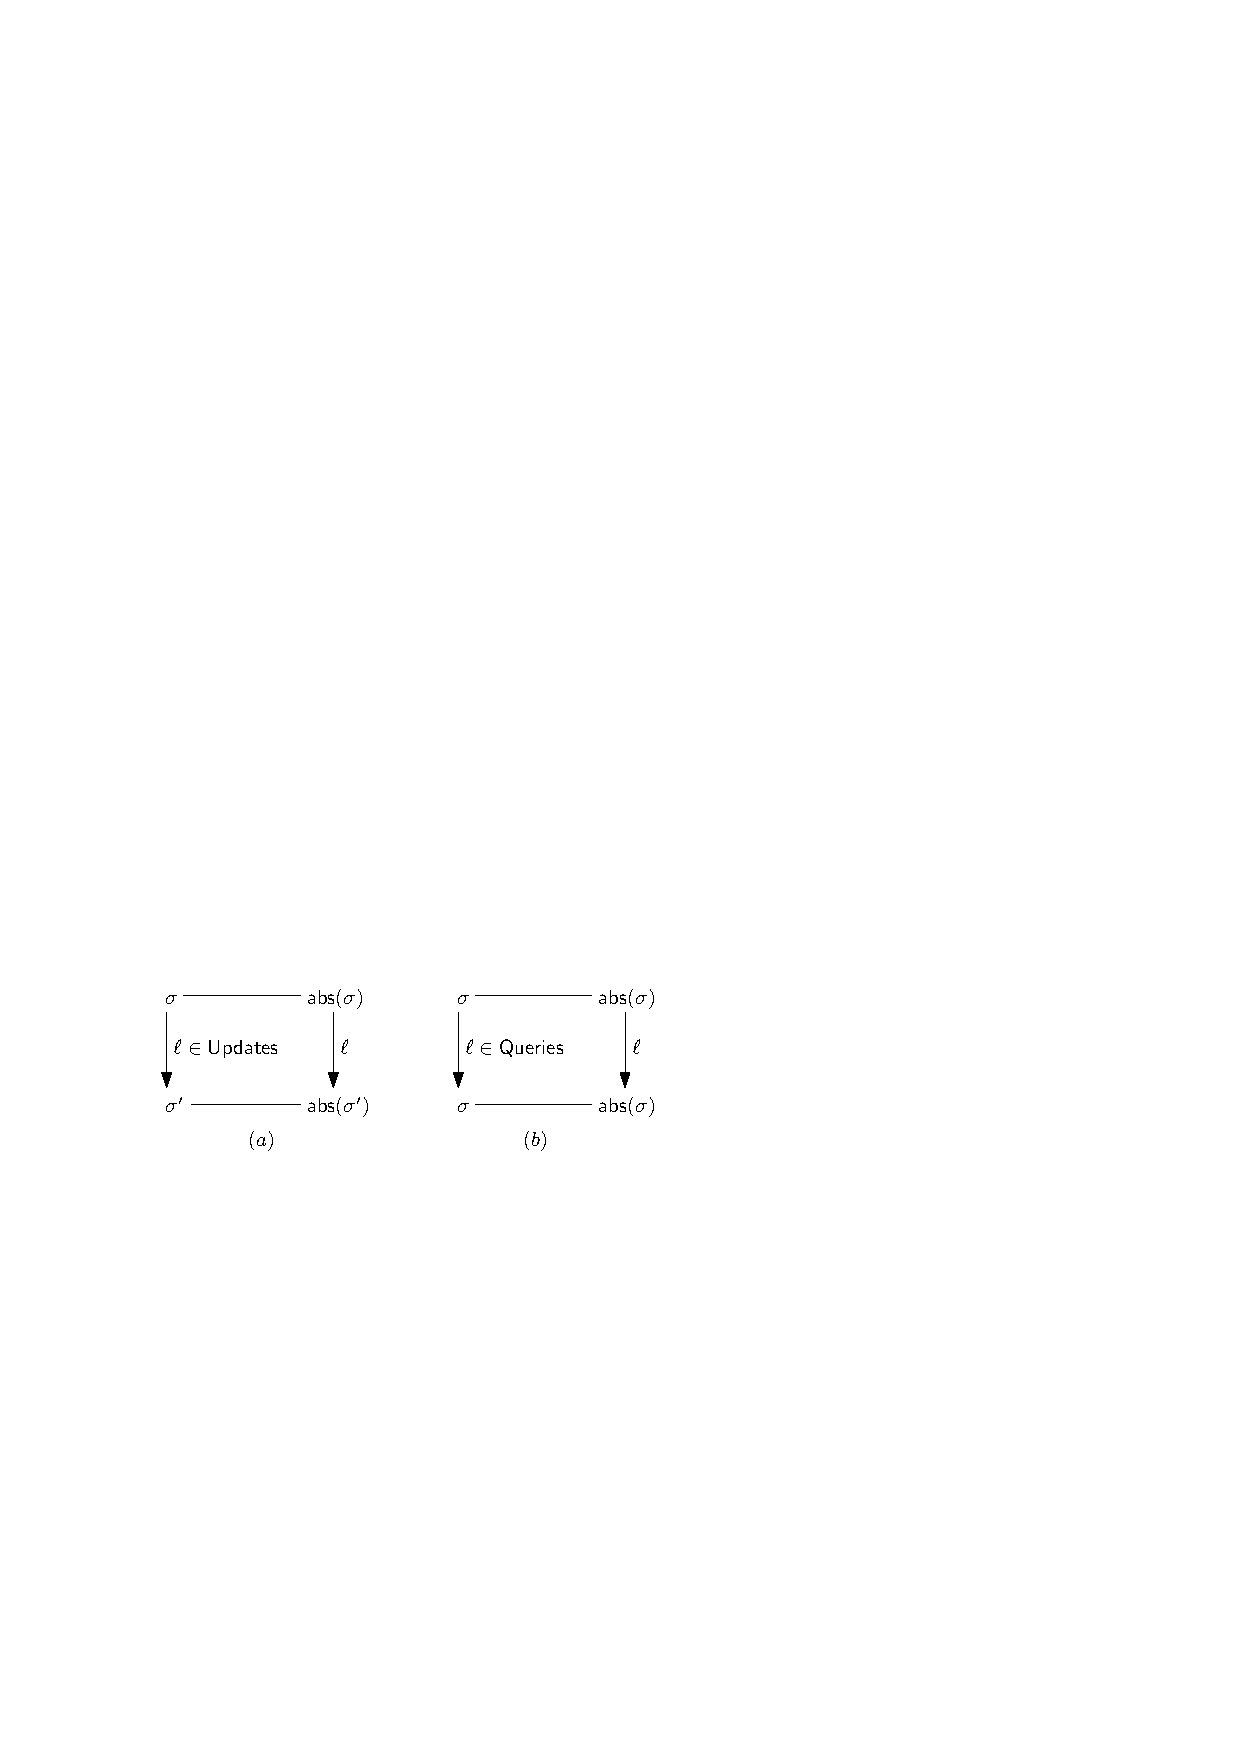
\includegraphics[width=0.8 \textwidth]{figures/RefinementMapping.pdf}
\vspace{-10pt}
  \caption{How refinement mapping works.}
  \label{fig:how refinement mapping works}
\end{figure}



\figurename~\ref{fig:an example of refinement mapping of an execution of RGA} gives an example of refinement mapping of an execution of RGA. Here we assume $\ats_a$ and $\ats_b$ is the timestamp of $a$ and $b$ respectively, and the timestamp order be $\ats_a < \ats_b$. Since applying downstream of concurrent operations commute, we take the order of ``increasing timestamp'': $\alabelshort[addAfter]{\circ,a} \cdot \alabelshort[addAfter]{\circ,a} \cdot \alabellong[read]{}{b \cdot a}{}$, and then, according to the refinement mapping, we construct the transitions in sequential specification.

\begin{figure}[t]
  \centering
  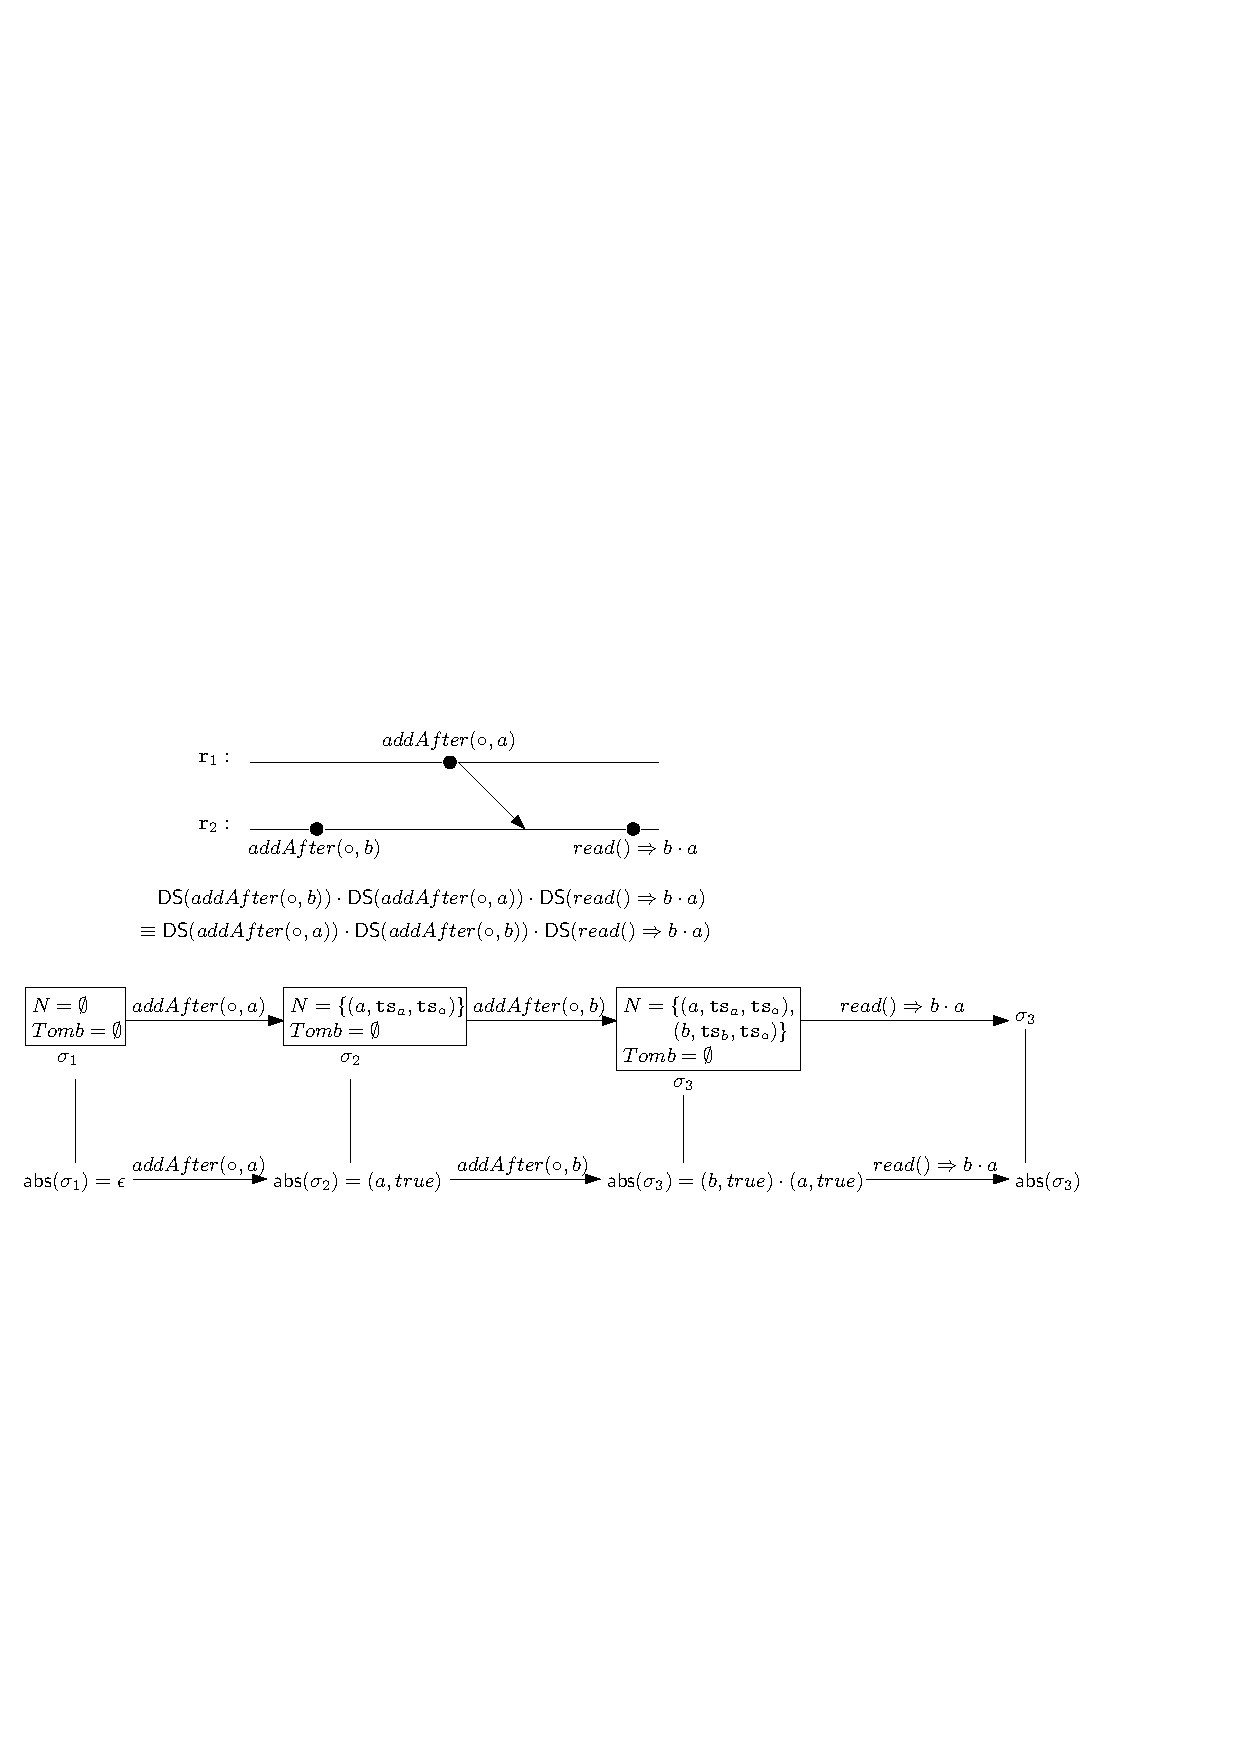
\includegraphics[width=0.85 \textwidth]{figures/RefinementMappingRGA.pdf}
\vspace{-10pt}
  \caption{An example of refinement mapping of an execution of RGA.}
  \label{fig:an example of refinement mapping of an execution of RGA}
\end{figure}



\figurename~\ref{fig:an example of refinement mapping of an execution of or-set} gives an example of refinement mapping of an execution of OR-set.

\begin{figure}[t]
  \centering
  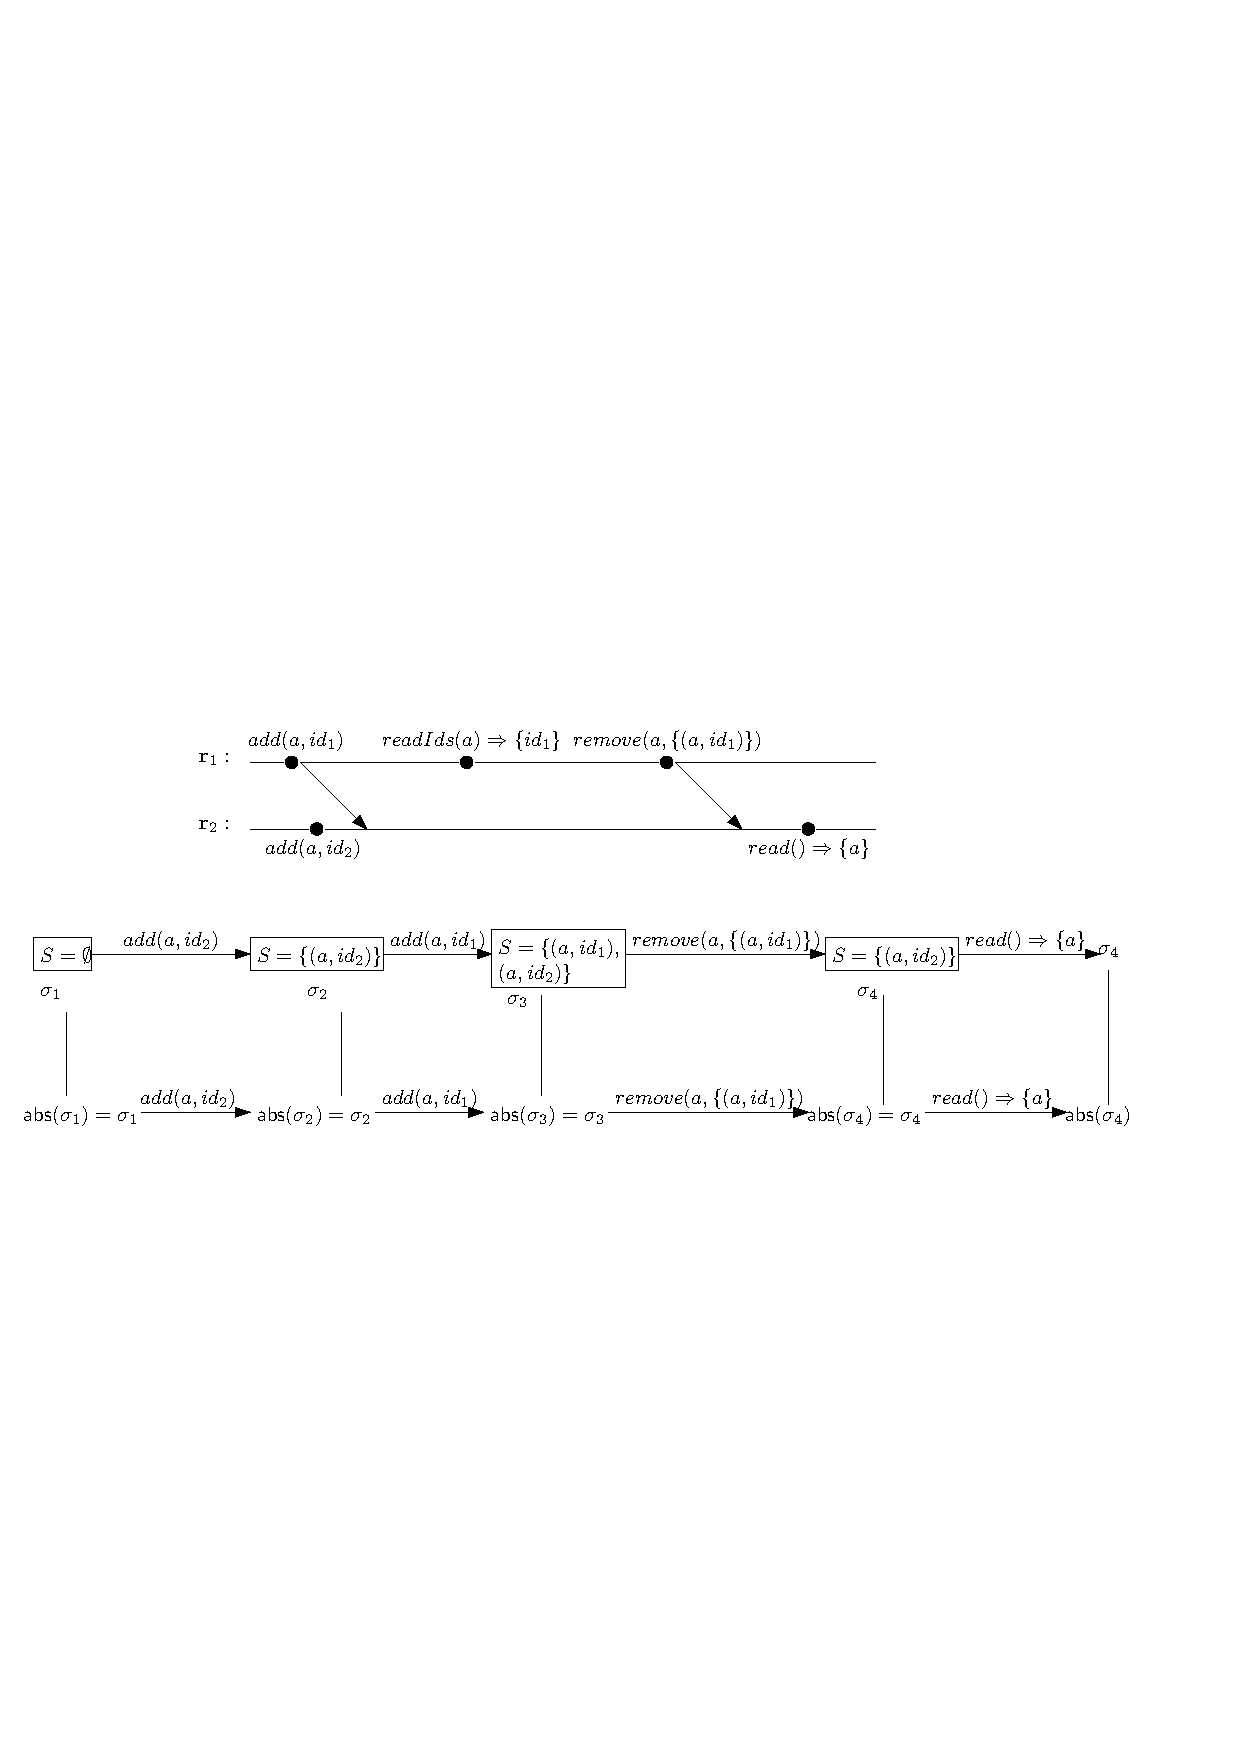
\includegraphics[width=0.85 \textwidth]{figures/RefinementMappingORSet.pdf}
\vspace{-10pt}
  \caption{An example of refinement mapping of an execution of OR-set.}
  \label{fig:an example of refinement mapping of an execution of or-set}
\end{figure}

%Let us consider another possible interface for RGA: $\alabelshort[{\tt addAt}]{a,k}$ puts value $a$ at the $k$-th position of the list, $\alabelshort[{\tt remove}]{a}$ removes a from the list, and $\alabellong[{\tt read}]{}{s}{}$ returns the list $s$. In \figurename~\ref{fig:an example that shows RGA with addAt interface is not compositional}, we show an example such that RGA with {\tt addAt} interface is not compositional. Here assume that timestamp order of $a,b$ is $a<b$, and the timestamp of $c,d$ is $c<d$. This history contains operations of two RGA objects $\aobj_1$ and $\aobj_2$, the operations of $\aobj_1$ being represented using blank circles and the operations of $\aobj_2$ using filled circles. The only possible \crdtlinearization{} of $\aobj_1$ is $\aobj_1.\alabelshort[{\tt addAt}]{a,1} \cdot \aobj_1.\alabelshort[{\tt addAt}]{b,2} \cdot \aobj_1.\alabelshort[{\tt remove}]{a}$; since in $\aobj_1.\alabelshort[{\tt addAt}]{a,1} \cdot \aobj_1.\alabelshort[{\tt remove}]{a} \cdot \aobj_1.\alabelshort[{\tt addAt}]{b,2}$, before inserting $b$, the list is $\epsilon$ and $b$ can not be inserted in position $2$. Similarly, the only possible \crdtlinearization{} of $\aobj_2$ is $\aobj_2.\alabelshort[{\tt addAt}]{c,1} \cdot \aobj_2.\alabelshort[{\tt addAt}]{d,2} \cdot \aobj_2.\alabelshort[{\tt remove}]{c}$. However, such two \crdtlinearization{} are not timestamp-order linearizations. Moreover, the two \crdtlinearization{} and the visibility relation berings a cycle.

%In \cite{DBLP:conf/podc/AttiyaBGMYZ16}, they use a more complex interface for RGA and other list implementations: $\alabellong[{\tt addAt}]{a,k}{s}{}, \alabellong[{\tt remove}]{a}{s}{},\alabellong[{\tt read}]{}{s}{}$: $\alabellong[{\tt addAt}]{a,k}{s}{}$ puts value $a$ in position $k$ of the list and returns the updated list $s$, $\alabellong[{\tt remove}]{a}{s}{}$ removes $a$ from the list and returns the updated list $s$, and $\alabellong[{\tt read}]{}{s}{}$ returns the list $s$. Similarly, such interface is not compositional.

%\begin{figure}[t]
%  \centering
%  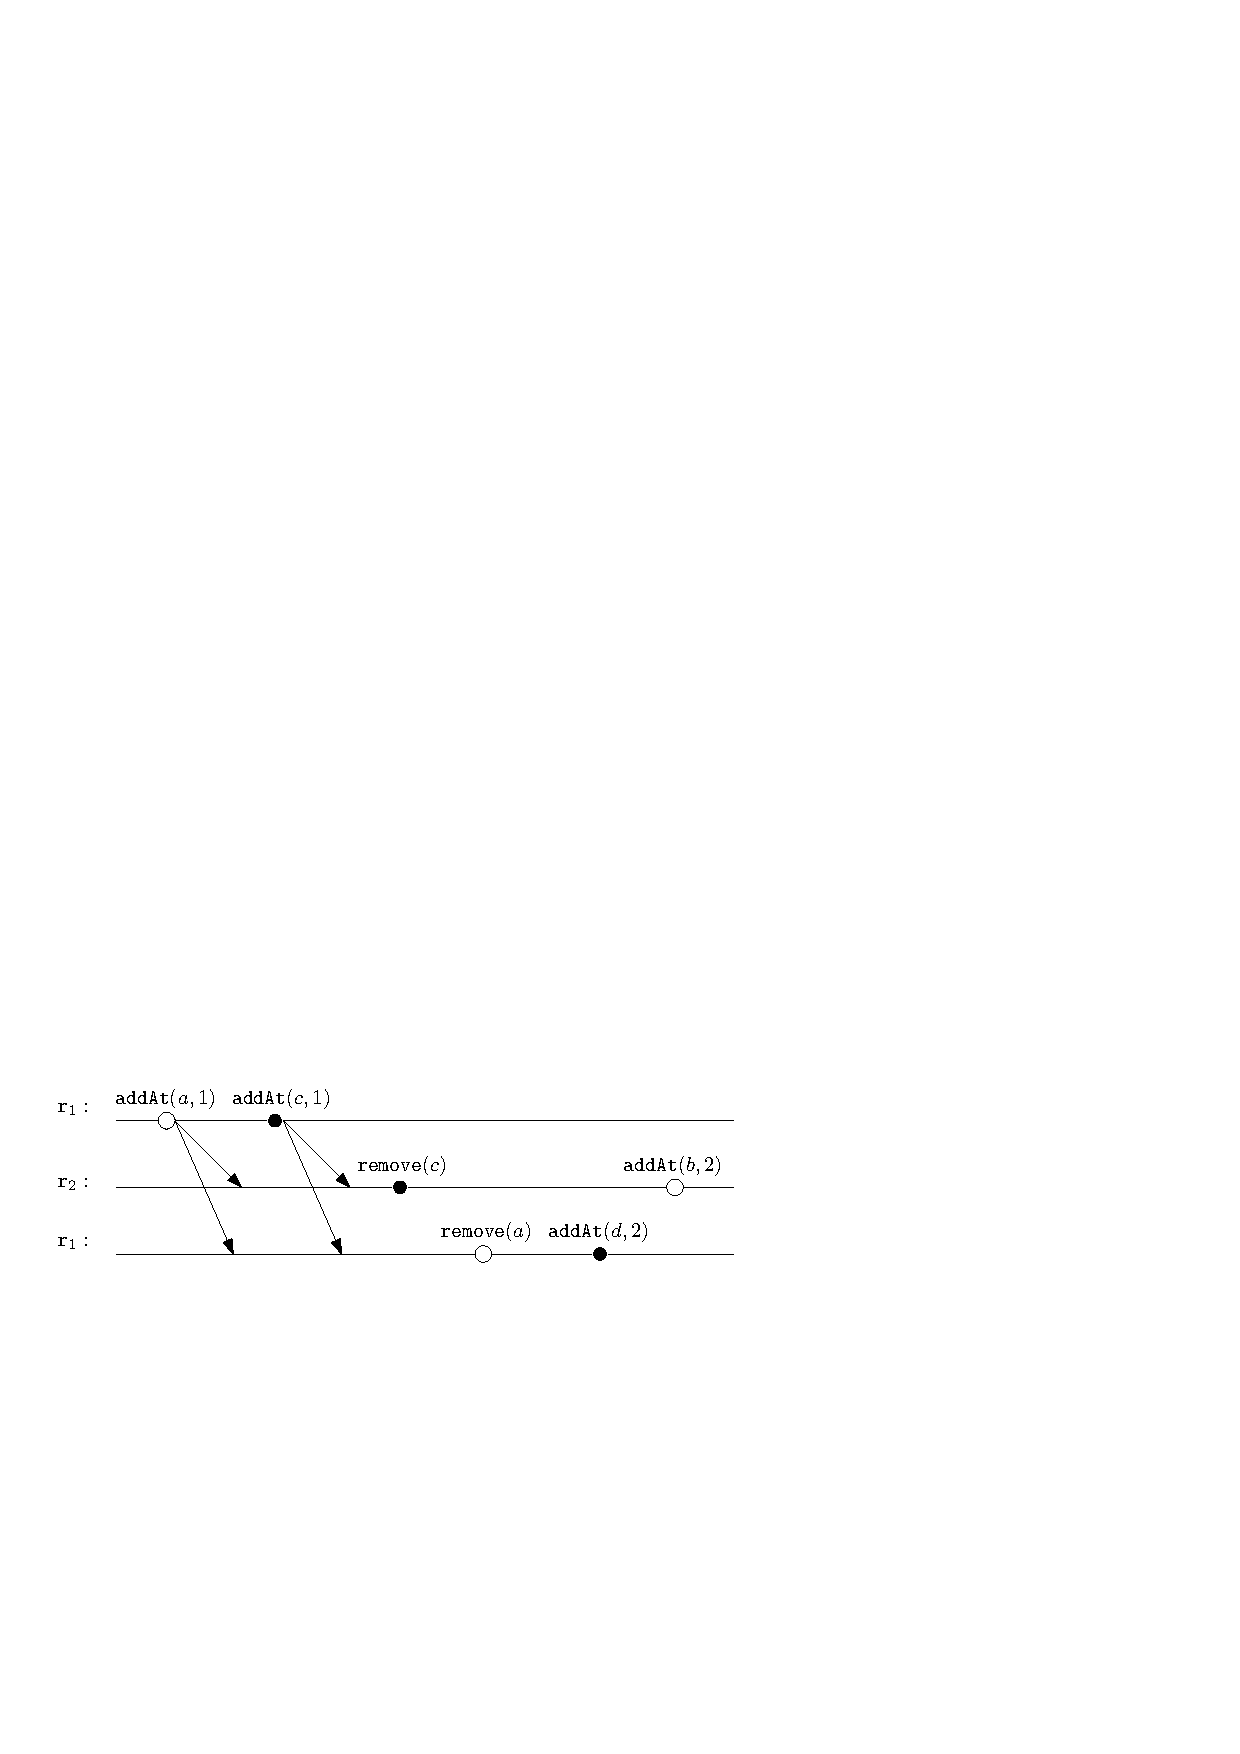
\includegraphics[width=0.85 \textwidth]{figures/RGAwithaddAtnotCompositional.pdf}
%\vspace{-10pt}
%  \caption{An example that shows RGA with {\tt addAt} interface is not compositional.}
%  \label{fig:an example that shows RGA with addAt interface is not compositional}
%\end{figure}



Let us consider another possible interface for RGA: $\alabelshort[{\tt addAt}]{a,k}$ puts value $a$ at the $k$-th position of the list, $\alabelshort[{\tt remove}]{a}$ removes a from the list, and $\alabellong[{\tt read}]{}{s}{}$ returns the list $s$. 

In \figurename~\ref{fig:an example that shows RGA with addAt interface is hard to prove}, we shows an example such that the proof of RGA with {\tt addAt} interface is hard to prove. Here assume that timestamp order of $b,c,d,e$ is $b<c<d<e$. Let us call the upper history $h_1$ and the history below $h_2$. The only difference between $h_1$ and $h_2$ is the position of $e$. Both $h_1$ and $h_2$ is \crdtlinearizable{}. However, their \crdtlinearization{} are completely different. We draw the \crdtlinearization{} below the corresponding history. This implies that, the \crdtlinearization{} is no longer timestamp-order linearizations, but something influenced by position. The position $2$ of $e$ in $h_2$ represents that ``the list contains at least one value'', which is essentially a semantics requirement, and it is reasonable to believe that the proof of RGA with {\tt addAt} interface will be much more complex than proving using timestamp-order linearizations.

\begin{figure}[t]
  \centering
  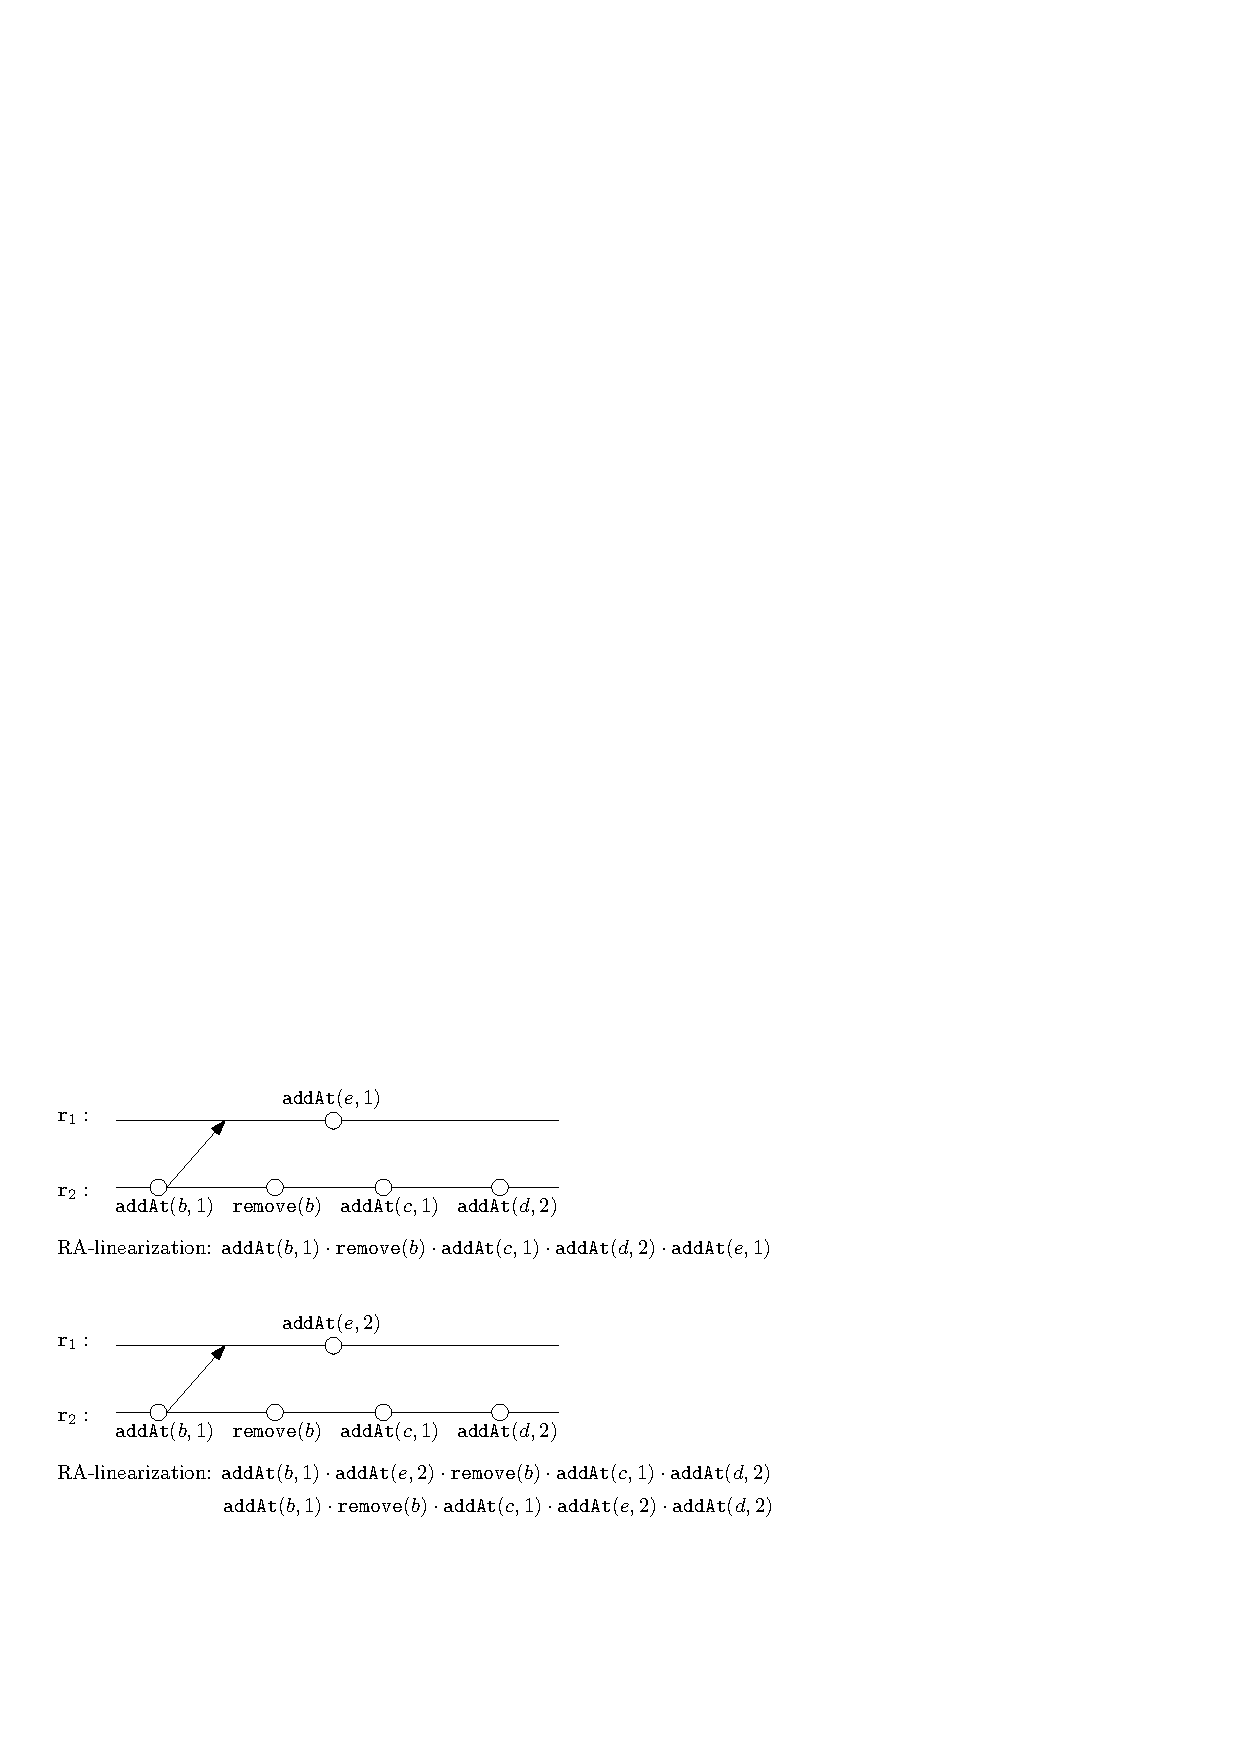
\includegraphics[width=0.7 \textwidth]{figures/RGAwithaddAtisHardtoProve.pdf}
\vspace{-10pt}
  \caption{An example that shows RGA with {\tt addAt} interface is hard to prove.}
  \label{fig:an example that shows RGA with addAt interface is hard to prove}
\end{figure} 


In \figurename~\ref{fig:an example that shows RGA with addAt interface is not RAlinearizable}, we shows an example of RGA, it uses {\tt addAt} interface, and is not \crdtlinearizable{}. Here assume that timestamp order of $a,b,c,d,e$ is $a<b<c<d<e$. For easy understanding, we also draw the local state of $\arep_3$ in \figurename~\ref{fig:an example that shows RGA with addAt interface is not RAlinearizable}. 

\begin{figure}[t]
  \centering
  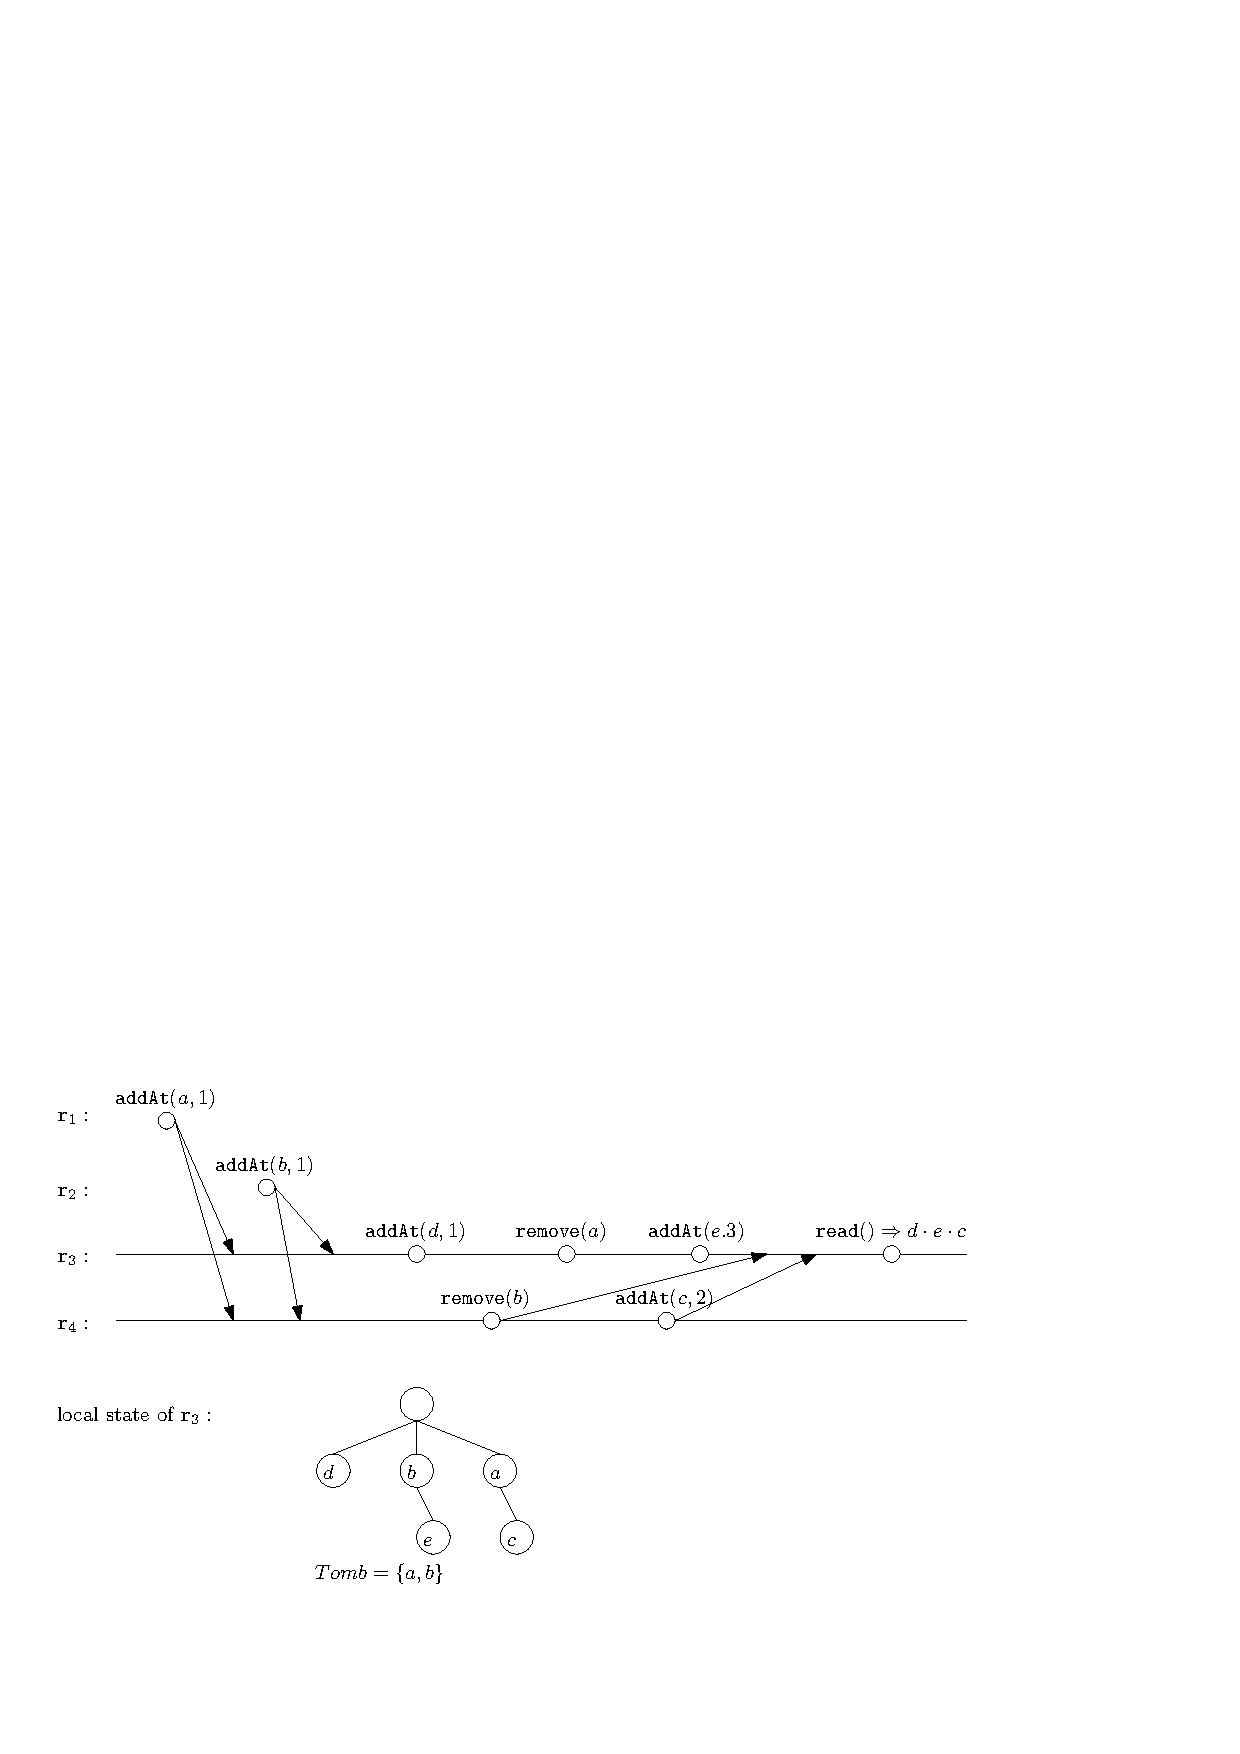
\includegraphics[width=0.7 \textwidth]{figures/RGAwithaddAtNotRALin.pdf}
\vspace{-10pt}
  \caption{An example that shows RGA with {\tt addAt} interface is not \crdtlinearizable{}.}
  \label{fig:an example that shows RGA with addAt interface is not RAlinearizable}
\end{figure} 


Therefore, we can see that, such {\tt addAt} interface is not suitable. In \cite{DBLP:conf/podc/AttiyaBGMYZ16}, they use a more complex interface for RGA and other list implementations: $\alabellong[{\tt addAt}]{a,k}{s}{}, \alabellong[{\tt remove}]{a}{s}{},\alabellong[{\tt read}]{}{s}{}$: $\alabellong[{\tt addAt}]{a,k}{s}{}$ puts value $a$ in position $k$ of the list and returns the updated list $s$, $\alabellong[{\tt remove}]{a}{s}{}$ removes $a$ from the list and returns the updated list $s$, and $\alabellong[{\tt read}]{}{s}{}$ returns the list $s$. Similarly, such interface has the above drawbacks. 


%The proof of $\mathsf{Refinement}$ relies on a \emph{refinement mapping}~\cite{AbadiL91} between replica states and states of the specification, denoted by $\refmap$. The proof goals require that for any two replica states $\sigma$ and $\sigma'$,
%\begin{enumerate}
%\item If $\sigma'$ is obtained from $\sigma$ by applying a downstream produced by an update $\alabel$: There exists a abstract $\refmap(\sigma')$ that is obtained from $\abstate_0$ by appling the downstreams of the operations in $\alabelset \cup \{ \alabel \}$ in the order defined by $\aseqord$.

%\item if a query $\alabel$ is applied on a state $\sigma$ or it is introduced by a rewriting of a query-update that executes {\tt atSource} on a state $\sigma$, then $\refmap(\sigma)\xRightarrow{\alabel}\refmap(\sigma)$.
%\end{enumerate}

%For the case of execution-order linearizations, the first case can be simplified into

%\begin{enumerate}
%\item if $\sigma'$ is obtained from $\sigma$ by applying a downstream $\delta$ produced by an update $\alabel$, then \mbox{$\refmap(\sigma)\xRightarrow{\alabel}\refmap(\sigma')$}, where $\xRightarrow{\alabel}$ is the transition function of $\Spec$.
%\end{enumerate}

%This simplification relies on proving concurrent operations commute.






























\forget{

\section{Compositionality of Distributed Linearizability}
\label{sec:compositionality of distributed linearizability}

\textblue{
This section should give three results of the form: if $o_1$ is linearizable w.r.t. $S_1$ and $o_2$ is linearizable w.r.t. $S_2$, and ???, then $o_1 \otimes o_2$ is linearizable w.r.t. $S_1\times S_2$ (the 2-object spec defined by interleavings). ??? may be an additional condition, while $\otimes$ is an "operator" for composing two CRDT implementations. Every result will have a different $\otimes$ operator.
\begin{itemize}
\item T0 + T0: ??? = $S_1$ and $S_2$ are $T0$-specs, and $\otimes$ is the trivial composition (the "unsynchronized" product)
\item T1 + T1: ??? = $S_1$ and $S_2$ are $T1$-specs, and $\otimes$ is the "shared counter" composition (the "unsynchronized" product with a restriction on the set of generated histories)
\item T0 + T1: ??? = $S_1$ is a $T_0$ spec, and $S_2$ is a $T1$-spec, and $\otimes$ is the "global causal delivery" composition (the "unsynchronized" product with a restriction on the set of generated histories)
\end{itemize}
Also, we should prove that composing two $T0$, resp., $T1$, specs results in a $T0$, resp., $T1$ spec, and composing a $T0$ with $T1$ results in a $T1$. With this, the extension to sets of objects is straightforward:  compose all $T0$ and independently, all $T1$, then compose the two resulting objects.}


\subsection{Definition of Compositionality}
\label{subsec:definition of compositionality}

The following is the definition of distributed linearizability for multi-object histories.

\begin{definition}[Distributed Linearizability for Multi-object Histories]
\label{definition:distributed linearizability for multi-object histories}
A multi-object history $h$ is \crdtlinearizable{}, if there exists a sequence $\mathit{lin}$, called linearization of $h$, such that

\begin{enumerate}[(i)]
\item The elements of $\mathit{lin}$ is generated from the operations of $h$: each operation $o = (m(a) \Rightarrow b,i,\mathit{obj})$ is transformed into $(m(a) \Rightarrow b,i,S)$ with $S$ set of identifiers of operations of visible to $o$ via $h.\mathit{vis}$.
\item $\mathit{lin}$ is consistent with $h. \mathit{vis}$.
\item For each object $\mathit{obj}$, $h \uparrow_{\mathit{obj}}$ is \crdtlinearizable{}, and $\mathit{lin} \uparrow_{ \mathit{obj} }$ is a \crdtlinearization{} of $h \uparrow_{\mathit{obj}}$.
\end{enumerate}

A set $H$ of multi-object histories are \crdtlinearizable{} w.r.t deterministic sequential specifications, if each of its history is.
\end{definition}

The following is the definition of compositional histories.

\begin{definition}[Compositionality]
\label{definition:compositionality}
A multi-object history $h$ is called compositional, if: $h \uparrow_{\mathit{obj}}$ is distributed linearizable for each object $\mathit{obj}$, if and only if, $h$ is distributed linearizable.
\end{definition}

It is easy to see that, a multi-object history $h$ being distributed linearizable implies that the projection of $h$ into each object is distributed linearizable. When proving compositionality, we only need to consider the opposite direction.




\subsection{T0-Linearizability and T1-Linearizability}
\label{subsec:t0-linearizability and t1-linearizability}

To prove compositional

T0-linearizability is a sub-class of distributed linearizability.

\begin{definition}[t0-linearizability]
\label{definition:t0-ilnearizability}
A single-object history $h$ is t0-linearizable w.r.t a sequential specification $\mathit{spec}$, if each sequence $\mathit{lin}$ shown below is a linearization of $h$ w.r.t $\mathit{spec}$:

\begin{itemize}
\setlength{\itemsep}{0.5pt}
\item[-] Each element $(\ell,i,\mathit{vis}^{-1}(i))$ of $\mathit{lin}$ is generated from an operation $(\ell,i,\_,\mathit{ts})$ of $h$.

\item[-] $\mathit{lin}$ is consistent with $\mathit{vis}$.
\end{itemize}
\end{definition}

To prove t0-linearizability, we introduce the notion of t0-specifications. A specification $\mathit{spec}$ is called t0-specification, if given a history $h$ that is distributed linearizable w.r.t $\mathit{spec}$, then any sequence that is consistent with visibility relation is a linearization of $h$.

The following lemma shows some sequential specifications are t0-specifications. Its proof can be found in Appendix \ref{subsec:appendix proofs of Lemma several t0-specifications}. Based on this lemma and our proofs in Section \ref{sec:proving distributed linearizability}, we can see that or-set is t0-linearizable w.r.t $\mathit{OR}$-$\mathit{set}_s$, and counter is t0-linearizable w.r.t $\mathit{counter}_s$.

\begin{restatable}{lemma}{SeveralTZeroSpecifications}
\label{lemma:several t0-specifications}
$\mathit{OR}$-$\mathit{set}_s$, $\mathit{set}_s$ and $\mathit{counter}_s$ are t0-specifications.
\end{restatable}



Given a history $h$, a sequence $\mathit{lin}$ is called a strict time-stamp order candidate of $h$, if for each elements $o_1,o_2$ of $\mathit{lin}$, if the time-stamp of $o_1$ in $h$ is less than that of $o_2$, then, $o_1$ is before $o_2$ in $\mathit{lin}$. T1-linearizability is a sub-class of distributed linearizability.

\begin{definition}[t1-linearizability]
\label{definition:t1-ilnearizability}
A single-object history $h$ is t1-linearizable w.r.t a sequential specification $\mathit{spec}$, if each strict time-stamp order candidiate $\mathit{lin}$ is a linearization of $h$.
\end{definition}

To prove t1-linearizability, we introduce the notion of t1-specifications. A specification $\mathit{spec}$ is called t1-specification, if given a history $h$ that is distributed linearizable w.r.t $\mathit{spec}$, and has a strict time-stamp order candidate as linearization, then any strict time-stamp order candidate is a linearization of $h$.

The following lemma shows some sequential specifications are t1-specifications. Its proof can be found in Appendix \ref{subsec:appendix proofs of Lemma several t1-specifications}. Based on this lemma and our proofs in Section \ref{sec:proving distributed linearizability}, we can see that RGA is t1-linearizable w.r.t $\mathit{list}_s^{\mathit{af}}$, and LWW-register is t1-linearizable w.r.t $\mathit{reg}_s$.

\begin{restatable}{lemma}{SeveralTOneSpecifications}
\label{lemma:several t1-specifications}
$\mathit{list}_s^{\mathit{af}}$ and $\mathit{reg}_s$ are t1-specifications.
\end{restatable}


\begin{table}
  \centering
  \begin{tabular}[t]{l|l}
    T0 & $\mathit{OR}$-$\mathit{set}_s$, $\mathit{set}_s$, $\mathit{counter}_s$,  \\
    T1 & $\mathit{list}_s^{\mathit{af}}$, $\mathit{reg}_s$,
  \end{tabular}
\end{table}




\subsection{Composing Several t0-Specifications}
\label{lemma:several t0-specifications can be composed}

The following lemma states that a history of several objects of t0 specifications is compositional. Its proof can be found in Appendix \ref{subsec:appendix proofs of lemma several t0-specifications can be composed}.

\begin{restatable}{lemma}{composingTZero}
\label{lemma:several t0-specifications can be composed}
Given a multi-object history $h$, if each of its object uses a t0-specification, then, $h$ is compositional.
\end{restatable}




\subsection{Composing Several t0-Specifications with One T1-specification}
\label{lemma:composing several t0-specification with one t1-specification}

Composing several t0-specifications with one t1-specification does not hold in general. \figurename~\ref{fig:a failed example of composing a multi-value register with a last-write-win register} is a history $h$ that is a failed example of composing a multi-value register with a last-write-win register, where the operations of LWW register are boxed. Here we assume that $\mathit{ts}_1<\mathit{ts}_2$. Since multi-value register is t0-specification and LWW register is t1-specification, we can see that the projection of $h$ into operations of multi-value register is distributed linearization and the only possible linearization is $\mathit{write}(a) \cdot \mathit{write}(b)$, and the projection of $h$ into operations of LWW register is distributed linearization and the only possible linearization is $\mathit{write}(c) \cdot \mathit{write}(d)$. However, $h$ is not distributed linearizable, since there is a a cycle.

\begin{figure}[t]
  \centering
  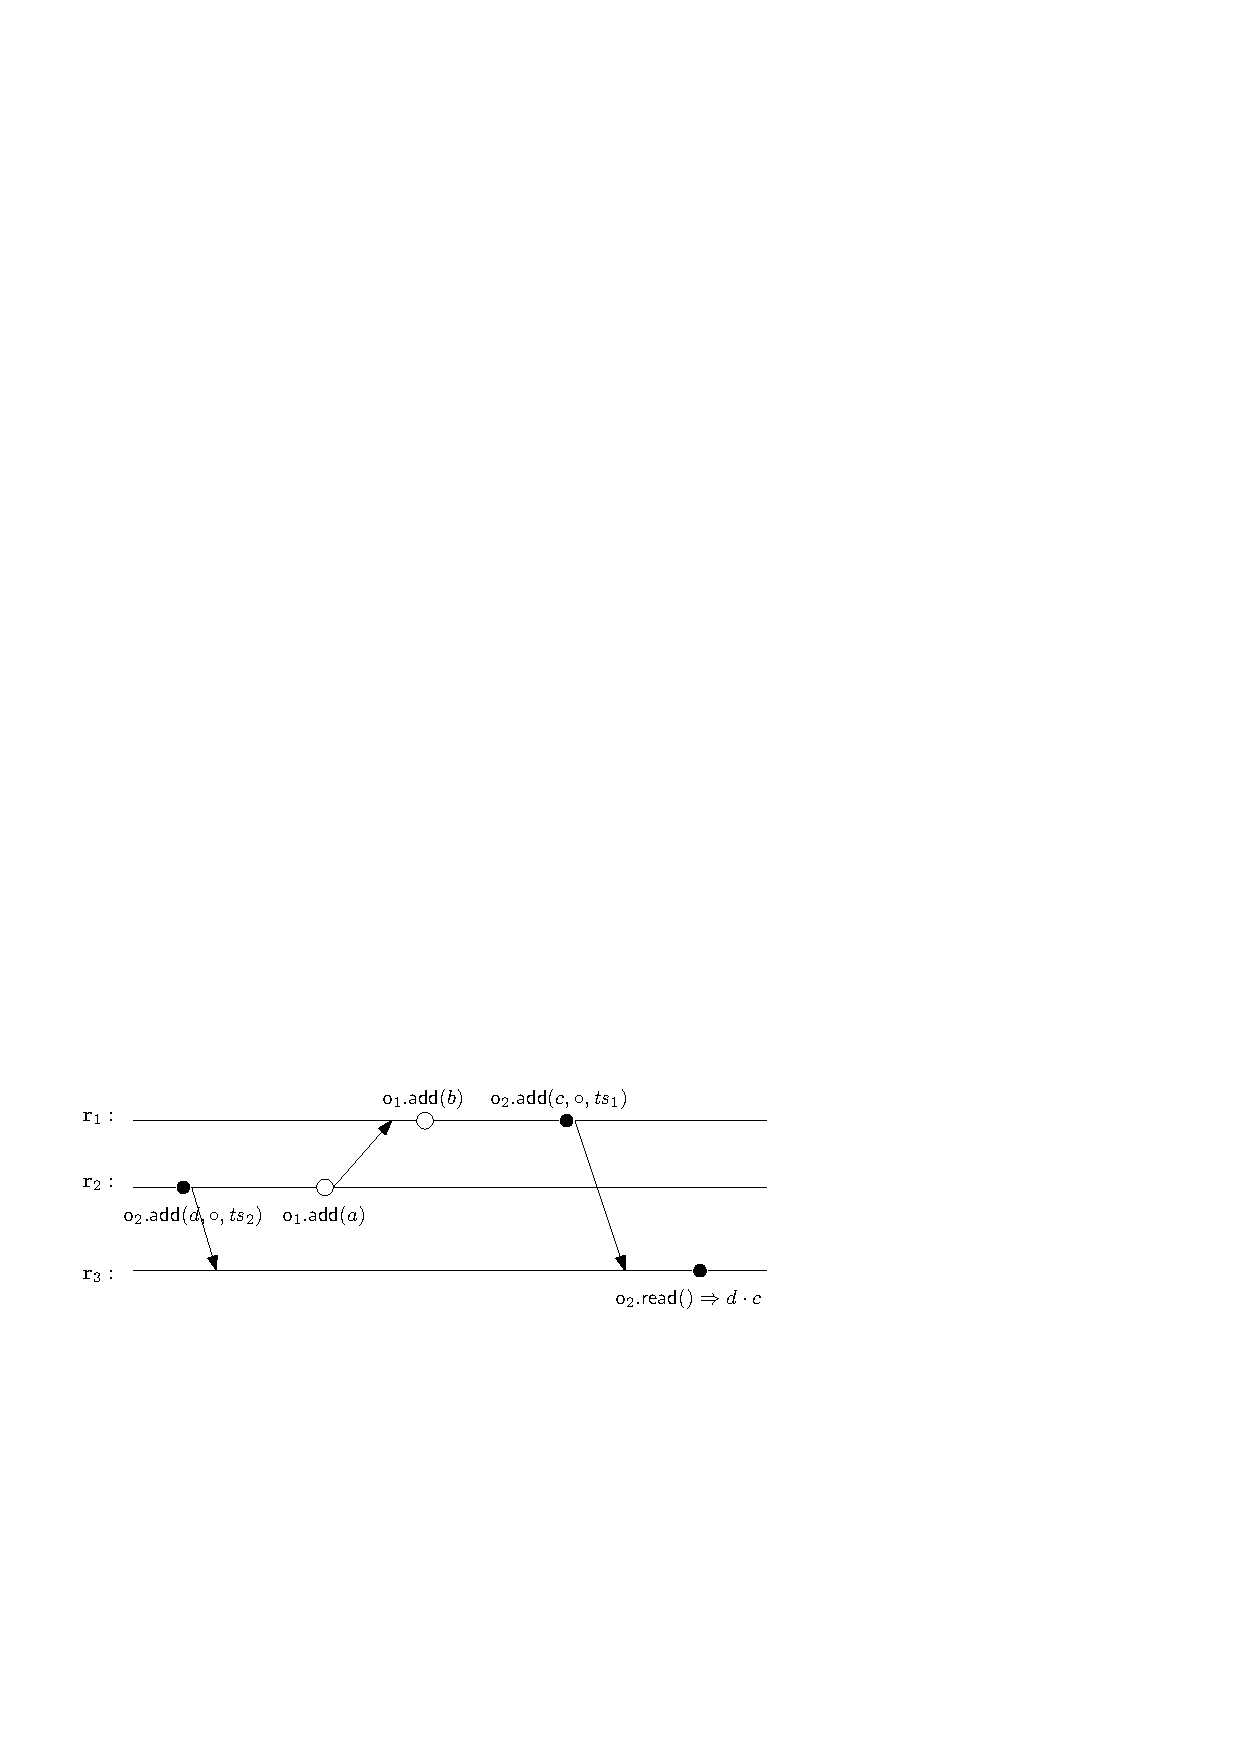
\includegraphics[width=0.6 \textwidth]{figures/MVReg-LWWReg-Nocd.pdf}
\vspace{-10pt}
  \caption{A failed example of composing a multi-value register with a last-write-win register (boxed operations), where $\mathit{ts}_1 < \mathit{ts}_2$.}
  \label{fig:a failed example of composing a multi-value register with a last-write-win register}
\end{figure}

The following lemma states that for a multi-object history, if its object use several t0-specifications and one t1-specification, and its visibility relation is transitive, then, $h$ is compositional. Its proof can be found in Appendix \ref{subsec:appendix proofs of lemma several t0-specifications and one t1-specification can be composed}.

\begin{restatable}{lemma}{composingTZeroAndOneTOne}
\label{lemma:several t0-specifications and one t1-specification can be composed}
Given a multi-object $h$, if its object use several t0-specifications and one t1-specification, and its visibility relation is transitive, then, $h$ is compositional.
\end{restatable}




\subsection{Composing Several t0-Specifications with Several T1-specification}
\label{lemma:composing several t0-specification with several t1-specification}

Composing several t0-specifications with several t1-specification does not hold in general. \figurename~\ref{fig:a failed example of composing two last-write-win registers} is a history $h$ that is a failed example of composing two last-write-win registers, where the operations of one LWW register are boxed, and the operations of the other LWW registers are not boxed. Here we assume that $\mathit{ts}_1 < \mathit{ts}_2 < \mathit{ts}_3$, and $\mathit{ts}'_1 < \mathit{ts}'_2$. Since LWW register is t1-specification, we can see that the projection of $h$ into operations of one LWW register is distributed linearization and the only possible linearization is $\mathit{write}(a,\mathit{ts}'_1) \cdot \mathit{write}(b,\mathit{ts}'_2)$, and the projection of $h$ into operations of the other LWW register is distributed linearization and the only possible linearization is $\mathit{write}(c,\mathit{ts}_1) \cdot \mathit{write}(d,\mathit{ts}_2) \cdot \mathit{write}(e,\mathit{ts}_3)$. However, $h$ is not distributed linearizable, since there is a a cycle.

\begin{figure}[t]
  \centering
  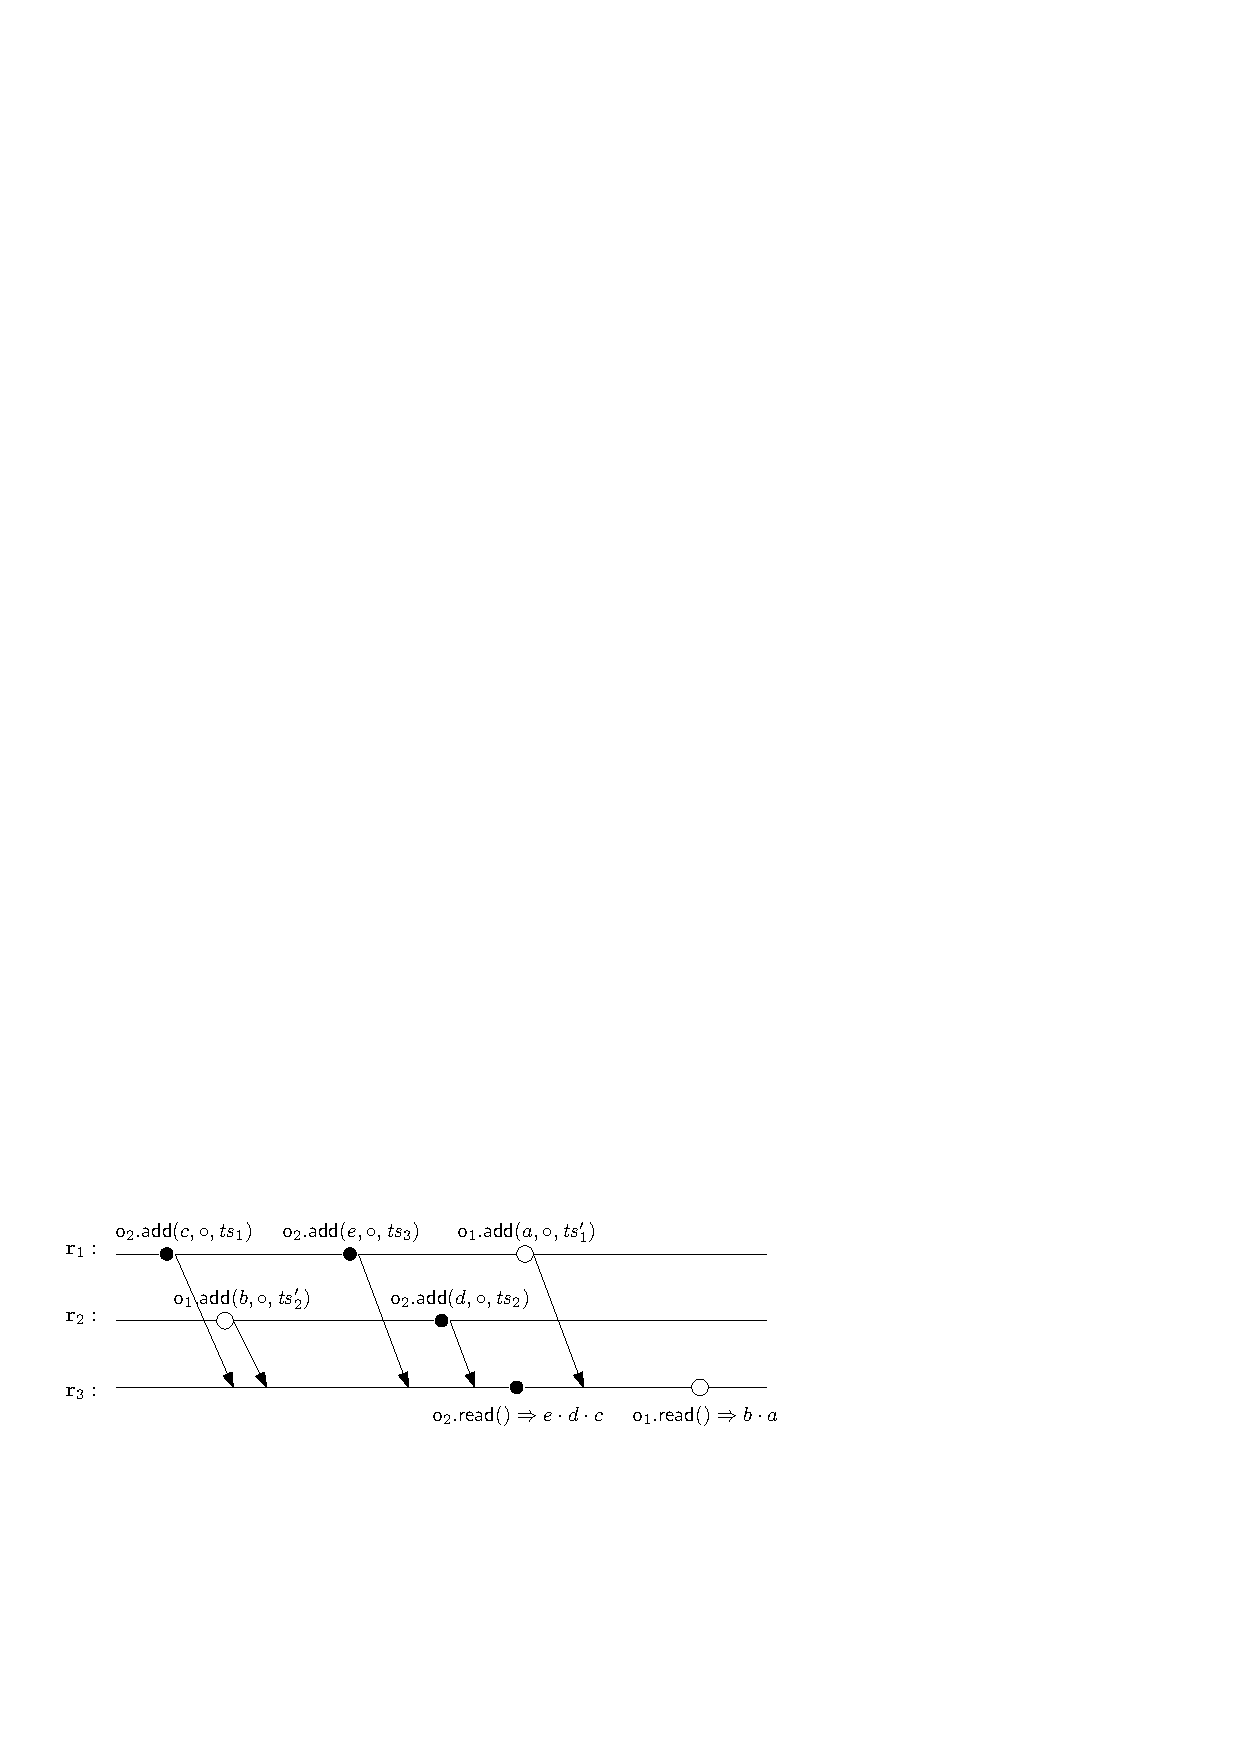
\includegraphics[width=0.7 \textwidth]{figures/LWWReg-LWWReg-NoSTS.pdf}
\vspace{-10pt}
  \caption{A failed example of composing two last-write-win registers (one object is boxed, the other is not), where $\mathit{ts}_1 < \mathit{ts}_2 < \mathit{ts}_3$, and $\mathit{ts}'_1 < \mathit{ts}'_2$.}
  \label{fig:a failed example of composing two last-write-win registers}
\end{figure}


A history $h$ satisfies causal-time-stamp, if: Given operation $o_1,\ldots,o_{\mathit{2k+2}}$ of $h$ that are of objects of t1-specification, if

\begin{itemize}
\setlength{\itemsep}{0.5pt}
\item[-] $(o_2,o_3)$ are of a same object, $\ldots$, $(o_{\mathit{2k}},o_{\mathit{2k+1}})$ are of a same object, $(o_{\mathit{2k+2}},o_1)$ are of a same object,

\item[-] $\mathit{ts}(o_2) < \mathit{ts}(o_2)$, $\ldots$, and $\mathit{ts}(o_{\mathit{2k}}) < \mathit{ts}(o_{\mathit{2k+1}})$,

\item[-] $(o_1,o_2), \ldots, (o_{\mathit{ek+1}},o_{\mathit{2k+2}}) \in \mathit{vis}$.
\end{itemize}

Then, we have $\mathit{ts}(o_1) < \mathit{ts}(o_{\mathit{2k+1}})$.

The following lemma states that for a multi-object history, if its object use several t0-specifications and several t1-specification, and it satisfies causal-time-stamp and its visibility relation is transitive, then, $h$ is compositional. Its proof can be found in Appendix \ref{subsec:appendix proofs of lemma several t0-specifications and several t1-specification can be composed}.

\begin{restatable}{lemma}{composingTZeroAndTOne}
\label{lemma:several t0-specifications and several t1-specification can be composed}
Given a multi-object $h$, if its object use several t0-specifications and several t1-specification, and it satisfies causal-time-stamp and its visibility relation is transitive, then, $h$ is compositional.
\end{restatable}






\subsection{Modified CRDT Implementation}
\label{subsec:modified CRDT implementation}

To ensure composing, we modify t1-algorithms as follows: The system supplies a method called $\mathit{updateGlobalTS}$, which supplies a time-stamp that is updated along the global system. When a method needs to generate new time-stamp, it calls this method to generate new time-stamp, and such process will also update the global time-stamp of this replica. When a method sends a message, the message should contain the current global time-stamp value. When a replica receives a message, it also use the global time-stamp value in message to update its own global time-stamp value. Moreover, the global time-stamp satisfies causal-time-stamp property.

The RGA algorithm after modification is as follows: Here a message contains the current global time-stamp value, and a replica update global time-stamp value is not explicitly written in code. Instead, such processes will be make explicit when constructing the operational semantics.

\begin{lstlisting}[caption={Pseudo-code of the Modified RGA}, captionpos=b,label={lst:modifier rga}]
  payload Ti-Tree N, Set Tomb
  initial N = @|$\emptyset$|@, Tomb = @|$\emptyset$|@

  addAfter(a,b) :
    atSource :
      precondition : b = @|$\circ$|@ or (b != @|$\circ$|@ and (b,_,_) @|$\in$|@ N and b @|$\not\in$|@ Tomb)
      let ts@|$_{\mathtt{a}}$|@ = updateGlobalTS()
      let ts@|$_{\mathtt{b}}$|@ = (b == @|$\circ$|@)?(0,r@|$_{0}$|@):(timestamp of b in N)
    downStream(a, ts@|$_{\mathtt{a}}$|@, ts@|$_{\mathtt{b}}$|@) :
      precondition: b = @|$\circ$|@ or (b != @|$\circ$|@ and (b, ts@|$_{\mathtt{b}}$|@,_) @|$\in$|@ N)
      N = N ts@|$\cup$|@ {(a, ts@|$_{\mathtt{a}}$|@, ts@|$_{\mathtt{b}}$|@)}

  remove(a) :
    atSource :
      precondition : a != @|$\emptyset$|@ and (a,_,_) @|$\in$|@ N and a @|$\notin$|@ Tomb
    downStream(a) :
      precondition : a != @|$\emptyset$|@ and (a,_,_) @|$\in$|@ N
      Tomb = Tomb @|$\cup$|@ {a}

  read() :
    return traverse(N, Tomb)
\end{lstlisting}


The following lemma states that the modified RGA is also t1-linearizable w.r.t $\mathit{list}_s^{\mathit{af}}$, and the modified LWW-register is t1-linearizable w.r.t $\mathit{reg}_s$. Its proof can be found in Appendix \ref{a}.

\begin{restatable}{lemma}{ModifiedRGAandLWWRegStillTOne}
\label{lemma:modified RGA and LWW-register is still t1-linearizable}
$\mathit{list}_s^{\mathit{af}}$ and $\mathit{reg}_s$ are t1-specifications.
\end{restatable}

Lamport's time-stamp is one way to implement global time-stamp, as stated by the following lemma. Its proof can be found in Appendix \ref{a}.

\begin{restatable}{lemma}{LamportTSasGlobalTS}
\label{lemma:lamport time-stamp as global time-stamp}
Lamport's time-stamp satisfies causal-time-stamp.
\end{restatable}








\subsection{Semantics of Multi Objects}
\label{subsec:semantics of multi objects}

When there is multiple objects, we say $(o_1,o_2) \in \mathit{vis}$, if either $(o_1,o_2) \in \mathit{ro}$, or $o_1$ is delivered to the replica of $o_2$ before $o_2$ happens. We consider CTDT implementation of t1-specifications use the time-stamp of Lamport's time-stamp: Each time-stamp is a tuple $(c,r)$ of a counter value $c \in \mathbb{N}$ and a replica identifier $r \in \mathbb{R}$; $(c_1,r_1) < (c_2,r_2)$, if $c_1 < c_2 \vee (c_1 = c_2 \wedge r_1 < r_2)$. To ensure compositionality of multiple objects, the following conditions needs to be satisfied:

\begin{itemize}
\setlength{\itemsep}{0.5pt}
\item[-] Cross-object-causal-delivery (COCD): We extend the notion of causal-delivery into multiple objects. Given two update operations $o_1$ and $o_2$, and assume $o_1$ is visible to $o_2$. Then, for each replica, once it receives $o_2$, it must be the case that $o_1$ has been previously received.

\item[-] Shared-time-stamp (STS): the objects of t1-specifications shares a counter $\mathit{sCtr}$. Each message carries a value of $\mathit{sCtr}$, and when generating new message, the value of $\mathit{sCtr}$ is also considered.
\end{itemize}



Based on shared-time-stamp,



Formally, given a set $\mathit{Objs}$ of objects, its semantics is defined as $\llbracket \mathit{Objs} \rrbracket_{\mathit{op}} = (\mathit{Config},\mathit{config}_0,\Sigma',\rightarrow)$ as in \figurename~\ref{fig:the semantics of multiple operation-based CRDT object}.


\begin{figure}[ht]
$\mathit{RState} = \mathit{Objs} \times \mathbb{R} \rightarrow \Sigma$

$\mathit{TState} = \mathbb{MID} \times \mathbb{MSG} \times \mathbb{R} \times \mathit{Objs}$

$\mathit{MsgHB} \subseteq \mathbb{MID} \times \mathbb{MID}$

$\mathit{MsgDel} \subseteq \mathbb{MID} \times \mathbb{R}$

$\mathit{Config} = \mathit{RState} \times \mathit{TState} \times \mathit{MsgHB} \times \mathit{MsgDel}$, $\mathit{config}_0 \in \mathit{Config}$.

$\Sigma' = \mathit{do}(\mathit{Objs} \times \mathbb{M} \times \mathbb{D} \times \mathbb{D} \times \mathbb{R} \times \mathbb{MID}) \cup \mathit{do}(\mathit{Objs} \times \mathbb{M} \times \mathbb{D} \times \mathbb{D} \times \mathbb{R}) \cup \mathit{receive}(\mathit{Objs} \times \mathbb{MID} \times \mathbb{R})$

\begin{itemize}
\setlength{\itemsep}{0.5pt}
\item[] $\begin{array}{l c}
   \bigfrac{
   \begin{array}{c}
     R(x,r) = \sigma, (x,r).\mathit{do}(\sigma,m,a) = (\sigma',b,\mathit{msg}), \mathit{msg} \neq \emptyset, \mathit{unique}(\mathit{mid}), \\
     S_1 = \{ (\mathit{mid}',\mathit{mid}) \vert (\mathit{mid'},r) \in \mathit{MsgDel} \}, S_2 = \{ (\mathit{mid}',\mathit{mid}) \vert \mathit{mid}' \in T, \mathit{mid}' \ is \ of \ replica \ r \}
   \end{array}}
     {(R,T,\mathit{msgHB},\mathit{MsgDel}) {\xrightarrow{\mathit{do}(x,m,a,b,r,\mathit{mid})}} (R[(x,r):\sigma'], T \cup \{ (\mathit{mid},\mathit{msg},r,x) \}, (\mathit{MsgHB} \cup S_1 \cup S_2)^*,\mathit{MsgDel})}
\end{array}$

\item[] $\begin{array}{l c}
   \bigfrac{
   \begin{array}{c}
     R(x,r) = \sigma, (x,r).\mathit{do}(\sigma,m,a) = (\sigma',b,\emptyset)
   \end{array}}
     {(R,T,\mathit{msgHB},\mathit{MsgDel}) {\xrightarrow{\mathit{do}(x,m,a,b,r)}} (R[(x,r):\sigma'], T \cup \{ (\mathit{mid},\mathit{msg},r) \}, \mathit{MsgHB},\mathit{MsgDel})}
\end{array}$

\item[-] $\begin{array}{l c}
   \bigfrac{
   \begin{array}{c}
      R(x,r) = \sigma, (x,r).\mathit{receive}(\sigma,\mathit{msg}) = \sigma', (\mathit{mid},\mathit{msg},r',x) \in T, r \neq r', \\
      (\mathit{mid},r) \notin \mathit{MsgDel}, \mathit{mid} \ is \ minimal \ w.r.t \ \mathit{MsgHB} \ among \ \{ \mathit{mid}' \vert (\mathit{mid}',r) \notin \mathit{MsgDel} \}
   \end{array}}
     {(R,T,\mathit{msgHB},\mathit{MsgDel}) {\xrightarrow{\mathit{receive}(x,\mathit{mid},r)}} (R,T,\mathit{MsgHB},\mathit{MsgDel} \cup \{ (\mathit{mid},r) \} )}
\end{array}$
\end{itemize}
\caption{The definition of semantics of $\llbracket \mathit{Objs} \rrbracket_{\mathit{op}}$}
\label{fig:the semantics of multiple operation-based CRDT object}
\end{figure}




$R$ is now a function from object and replica identifier to local state. Message and action also record its object. $\mathit{MsgHB}$ and $\mathit{MsgDel}$ now record the relation between messages of multiple objects. In each transition rule of \figurename~\ref{fig:the semantics of multiple operation-based CRDT object}, we deal with each object according to its CRDT implementations. Similarly, a sequence $l$ of actions is an execution of $\llbracket \mathit{Objs} \rrbracket_{\mathit{op}} = (\mathit{Config},\mathit{config}_0,\Sigma',\rightarrow)$, if there exists $(R,T,\mathit{MsgHB},\mathit{MsgDel}) \in \mathit{Config}$, such that $\mathit{config}_0 {\xrightarrow{ l }} (R,T,\mathit{MsgHB},\mathit{MsgDel})$. The semantics of $\mathit{Objs}$ is defined as the set of executions of $\llbracket \mathit{Objs} \rrbracket_{\mathit{op}}$.





A configuration $(R,T,\mathit{MsgHB},\mathit{MsgDel})$ is a snapshot of distributed system. $R$ gives the local state of each replica, and $T$ gives the set of messages that has been generated. Let $\mathbb{MID}$ be the set of message identifiers of message content. A message is a tuple $(\mathit{mid},\mathit{msg},r)$, where $\mathit{mid} \in \mathbb{MID}$ is the identifier, $\mathit{msg} \in \mathbb{MSG}$ is the message content, and $r$ is the original replica of message. $\mathit{MsgHB}$ is used to record the happen-before relation between messages: two messages $(\mathit{mid}_1,\mathit{mid}_2) \in \mathit{MsgHB}$ represents that the operation of $\mathit{mid}_1$ happens before the operation of $\mathit{mid}_2$. $\mathit{MsgDel}$ is used to record the message delivery relation between messages: $(\mathit{mid},r) \in \mathit{MsgDel}$ represents that message $\mathit{mid}_1$ has already been delivered to replica $r$. $\mathit{MsgHB}$ and $\mathit{MsgDel}$ are used to ensure message delivery requirements. $\mathit{config}_0$ is the initial configuration, which maps each replica into the initial local state, has no message, and with a empty happen-before relation and a empty message delivery relation.


Each element of $\Sigma'$ is called an action. $\rightarrow \in \mathit{Config} \times \Sigma' \times \mathit{Config}$ is the transition relation and describes a single step of distributed systems. The first rule in \figurename~\ref{fig:the semantics of a operation-based CRDT object} describes replica $r$ performs a update operation $m(a) \Rightarrow b$ and generates a message with message content $\mathit{msg}$. Here $\mathit{unique}$ is a function that ensures $\mathit{mid}$ be a fresh message identifier. We insert message identifier $\mathit{mid}$ into the happen-before relation and keeps the happen-before relation be transitive. The second rule describes replica $r$ performs a query operation $m(a) \Rightarrow b$ and thus does not generate message. Since no message is generated, the $\mathit{MsgHB}$ and $\mathit{MsgDel}$ tuples remain the same. The third rule describes delivery of a message to a replica $r$ other than its origin replica $r'$. By $(\mathit{mid},r) \notin \mathit{MsgDel}$, we ensure that $\mathit{mid}$ has not been previously delivered to replica $r$, and thus, each message be delivered to each replica at most once. By $\mathit{mid}$ being minimal w.r.t $\mathit{MsgHB}$ among $\{ \mathit{mid}' \vert (\mathit{mid}',r) \notin \mathit{MsgDel} \}$, we always choose a minimal element w.r.t $\mathit{MsgHB}$ among operations not been delivered to a replica, and thus, ensures causal-delivery.



\subsection{Proving in Multi-Objects Semantics}
\label{subsec:proving in multi-object semantics}


The formation of CRDT in this semantics is changed as follows,

The CRDT proved distributed linearizable are still distributed linearizable in this new semantics.
}

%%% Local Variables:
%%% mode: latex
%%% TeX-master: "draft"
%%% End:


%%% Local Variables:
%%% mode: latex
%%% TeX-master: "draft"
%%% End:
